\documentclass[12pt]{article}
\usepackage[margin=1in]{geometry}
\usepackage{amsmath,amssymb}
\usepackage{graphicx}
\usepackage{booktabs}
\usepackage{tabularx}
\usepackage{xcolor}
\usepackage{hyperref}
\setcounter{secnumdepth}{0}
\usepackage{amsmath,amssymb,amsfonts}
\usepackage{algorithm}
\usepackage{algorithmic}
\usepackage{tikz}
\usetikzlibrary{arrows.meta,positioning,shapes.geometric}
\usepackage{float}
\usepackage{graphicx}
\usepackage{fullpage}
\DeclareUnicodeCharacter{202F}{~} % Replaces narrow no-break space with LaTeX non-breaking space


\title{Algorithmic Collusion in Auctions: Evidence from Controlled Laboratory Experiments}
\author{Pranjal Rawat}
\date{\today}

\begin{document}

\maketitle

\begin{abstract}
Algorithms are increasingly being used to automate participation in online markets. Banchio and Skrzypacz (2022) demonstrate how exploration under identical valuation in first-price auctions may lead to spontaneous coupling into sub-competitive bidding. However, it is an open question if these findings extend to affiliated values, optimal exploration, and specifically which algorithmic details play a role in facilitating algorithmic collusion. This paper contributes to the literature by generating robust stylized facts to cover these gaps. I conduct a set of fully randomized experiments in a controlled laboratory setup and apply double machine learning to estimate granular conditional treatment effects of auction design on seller revenues. I find that first-price auctions lead to lower seller revenues and higher seller regret under identical values, affiliated values, and under both Q-learning and Bandits. There is more possibility of such tacit collusion under fewer bidders, Boltzmann exploration, asynchronous updating, and longer episodes; while high reserve prices can offset this. This evidence suggests that programmatic auctions, e.g. the Google Ad Exchange, which depend on first-price auctions, might be susceptible to coordinated bid suppression and significant revenue losses.
\end{abstract}

% Main sections
\newpage
\section{Introduction}

Intelligent algorithms are rapidly taking over real-time computerized auctions and markets in areas such as online marketplaces for pre-owned items, display advertising, sponsored search, financial trading, electricity, transportation, and public procurement. Significant concerns arise about the efficiency of auctions—originally tailored to human participants—under this new regime of algorithmic bidding. For instance, in large-scale advertising exchanges like Google AdSense, even minor inefficiencies or bid suppression can cause million-dollar losses. Recent work on algorithmic collusion in auctions has established that reinforcement-learning agents can spontaneously converge to sub-competitive bidding patterns. Calvano et al. (2020) demonstrate this phenomenon in pricing games, while Klein (2021) extends the analysis to sequential pricing with Q-learning. Banchio and Skrzypacz (2022) examine first- versus second-price auctions, finding that the former is more prone to bid suppression under simple Q-learning. However, these studies focus on narrow settings (constant valuations, small numbers of bidders, simple exploration mechanisms) and do not systematically parse how algorithmic factors (learning rates, discount factors, synchronization modes, budget constraints) amplify or mitigate tacit collusion.

This leaves open important questions: Do these findings hold when bidders have stochastic, possibly affiliated valuations? Are the results sensitive to the fine details of the algorithm? Are conclusions sensitive to different ways of exploring or initializing Q-values? Would the results change if algorithms explored the bid space in a more efficient way? What is the role of competitive pressure and informtion disclosures? Empirical data on real-world algorithmic auctions are fairly inaccessible, as most auctions are proprietary. Theoretical work also faces challenges, since modeling high-dimensional dynamic systems of Q-learning agents is analytically intractable. Indeed, if they were transparent then we would not have to wait until 2017 for Q-learning to attain superhuman prowess in chess. Existing theoretical papers typically focus on small state/action spaces and very crude learning algorithms.

This is where experimental work can come in and shed light on machine behaviour in important settings. However, experimental work in this area has also been partial in scope, rarely examining multiple interacting factors (e.g., discounting, asynchronous updates, alternative exploration strategies). This paper adopts a rigorous statistical approach and documents important facts about algorithmic learning in repeated auctions. A parallel literature examines budget-constrained bidding and pacing algorithms in online advertising auctions. Conitzer et al. (2022) characterize pacing equilibria in first-price auction markets and show that multiplicative pacing can lead to inefficient outcomes. Balseiro and Gur (2019) develop dual-based pacing algorithms that converge to near-optimal spending policies, though their analysis assumes stationary environments. Recent work on the price of anarchy in repeated auctions quantifies welfare losses when bidders optimize inter-temporally under budget constraints. This literature focuses on algorithm efficiency and convergence properties but does not examine collusion or strategic bid suppression. This paper addresses the gap by conducting a fully randomized factorial experiment comprising four experiments, each involving hundreds of independent trials and up to 100,000 simulated auctions per trial. Bidders apply reinforcement learning or bandit-based exploration under varied institutional elements (e.g., private vs.\ affiliated values, number of bidders, reserve prices) and algorithmic parameters (e.g., discount factors, Q-learning rates, synchronous vs.\ asynchronous updates, different exploration rules).

This paper offers one of the most comprehensive experimental studies of algorithmic learning in sealed-bid auctions to date, examining an exceptionally wide range of parameters and outcomes. We systematically investigate Q-learning, contextual bandits, and budget-constrained pacing algorithms, incorporate affiliated values to capture the continuum between private and common values, and measure not only revenue and regret but also price volatility, no-sale rates, and winner identity patterns. By varying reserve prices, the number of bidders, exploration schemes (Boltzmann vs.\ $\varepsilon$-greedy, synchronous vs.\ asynchronous Q-learning), and budget constraints, we uncover robust heterogeneity and interactions between auction formats and algorithmic details. More broadly, this paper demonstrates how factorial design methodology can efficiently analyze machine behavior in controlled environments, yielding interpretable main effects and interaction terms that generalize across learning paradigms.

Across all four experiments, I establish that first-price auctions consistently exhibit coordinated bid suppression, while second-price auctions align winning bids more closely with actual valuations and reduce volatility during the learning phase. This pattern is robust to valuation structure (constant vs.\ affiliated), learning algorithm (Q-learning, LinUCB, pacing controllers), and budget regime (unconstrained vs.\ constrained). The factorial analysis reveals heterogeneous treatment effects: the revenue loss from first-price auctions is magnified by fewer bidders, higher discount factors, asynchronous updating, and tighter budget constraints, while reserve prices provide partial mitigation. A distinctive feature of this paper is the systematic comparison across all four experiments to distinguish robust patterns from context-dependent effects. Section~\ref{sec:discussion} synthesizes findings across Q-learning (Experiments~1--2), contextual bandits (Experiment~3), and budget-constrained pacing (Experiment~4), identifying which mechanisms generalize across all settings and which vary by algorithmic paradigm. This cross-experiment framework reveals that first-price underperformance is universal, while the magnitude of revenue loss and the efficacy of moderating factors (exploration, competition, budget constraints) depend critically on algorithm class and valuation structure. The discussion provides quantitative comparisons of convergence speed, revenue gaps, and the role of exploration mechanisms across all experiments, establishing a taxonomy of robust versus algorithm-specific findings.

\section{Literature}

There are a few kinds of literature that are relevant. First, a theoretical literature on auctions that assumes rational actors. Second, an experimental literature replaces rational actors with humans or algorithms. Third, empirical evidence on algorithmic adoption and collusion. Fourth, legal literature on possible gaps in regulation. 

The first thread is theoretical literature on auctions (Milgrom and Weber 1982, Krishna 2009). The second price auction is superior to the first price auction when bidders only have a noisy signal about the actual value of the item. The first price auction suffers from the risk of the winner's curse, which leads to conservative bidding, and this reduces auction revenues. These results can break down in repeated games, and the Folk Theorem says that if bidders are patient enough, any average winning bid can be supported by a suitable and credible threat of punishment e.g., tit-for-tat or grim trigger. Tacit collusion in repeated auctions will take the form of symmetrically suppressed bids or asymmetric bid rotation. 

Oligopoly theory also offers some insight into the determinants of tacit collusion in repeated games. Ivaldi et al. (2002) show that in repeated games, the degree of tacit collusion rises with a higher discount rate, fewer market participants, symmetric conditions, higher entry barriers, a high frequency of interaction, greater transparency, and data availability. The last three factors are magnified with algorithms and are often cited as the reason for concern for algorithmic collusion. 

The second thread consists of experiments. The experimental evidence with humans shows a distinctive departure from theory (Kagel and Levin 2011). Bids are generally above Nash prediction in both the first and second price auctions. Experiments with noisy signals show a significant presence of the winner's curse, which even experienced bidders are unable to avoid (Levin et al., 1996). Sequential auctions of identical items often show declining prices (Keser et al., 1996, Neugebauer et al., 2007). 

Experiments with algorithms have highlighted different mechanisms through which tacit collusion can occur. Waltman and Kamyak (2008), Dopologov (2021) and Abada et al (2022) show how certain exploration strategies can lead to collusive outcomes. Asker et al (2021) highlight asynchronous vs synchronous learning. Calvano (2020) studies retaliatory strategies in simultaneous pricing games. Klein (2021) studies sequential pricing games and granularity of action spaces. Hansen et al (2021) study collusion arising from misspecified prediction and correlated price experimentation. Hettich (2021), Han (2022) and Zhang (2021) study deep reinforcement learning and compare different sampling strategies. Most of the literature on algorithmic collusion has focused on pricing and the only experiments with auctions can be found in Banchio and Skrzypacz (2022).

A few papers look at algorithms learning to bid in auctions. Bandyopadhyay et al. (2008), study reverse auctions with reinforcement learning and find that in simple cases mixed strategy equilibrium can be attained. Tellidou et al.,(2007) study electricity markets and find that tacit collusion is easy to sustain even under competitive conditions. Banchio and Skrzypacz (2022) study auction design with Q-learning bots and found that the first price auction can lead to collusive outcomes while the second price auction does not. Criticisms of simulation-based studies are that settings are too stylized, using competitive rather than monopolistic benchmarks is unrealistic, and algorithms tested are too unrealistic (Kühn \& Tadelis 2017, Schwalbe 2018).

The third thread looks at the pervasive adoption of algorithms and actual evidence for algorithmic collusion. Chen et al. (2016) studied 1,641 best-seller products on Amazon and detected that about 543 had adopted some form of algorithmic pricing. A 2017 OECD report titled ``Algorithms and Collusion" found that \textit{``Two-thirds of them [ecommerce firms] use automatic software programs that adjust their own prices based on the observed prices of competitors"}. A 2023 eMarketer report shows that algorithms are dominating bidding in display and sponsored search auctions across the globe. Brogaard et al., (2014) find that algorithms have come to dominate trading in the double auction markets. 

These developments have led to limited evidence of algorithmic collusion. Assad et al. (2020) study the adoption of algorithmic pricing in German gasoline markets. They find that adoption increases margins by 9\% in competitive markets and upto 28\% in duopolies. Brown and Mackay (2021) five largest online retailers in over-the-counter allergy medications. The use of automated software to change prices quickly leads to prices that are 10 percent higher than otherwise. Musoloff (2022) studied data from Amazon Marketplace and found that adopting algorithmic pricing reduces prices on average but leads to ``resetting" price cycles where participants regularly increase prices at night to cajole the others into following suit. We also see a few legal cases already. \footnote{The 2015 Topkins (US) and 2016 GB Posters (UK) cases brought to light price fixing via pricing algorithms on Amazon. In 2018, after the insolvency of Air Berlin, Lufthansa abused its temporary monopoly power by raising prices roughly by 25\% through pricing algorithms. In 2021, Google was fined 2.42 billion Euro for using algorithms to exclusively place its own Shopping services on Google search while demoting rival providers. Similarily, Amazon is currently defending a claim that its algorithms put its own products over rivals on its lucrative ‘Featured Offer’ placement. There have also been hub-and-spoke conspiracies. In 2016, e-Turas the Lithuanian travel website, was charged for imposing caps on discount rates proposed by travel agencies. In 2018, Accenture was accused of using its software Partneo to coordinate price increases on auto parts, dramatically increasing revenue for major carmakers.}

The fourth thread looks at possible gaps in regulation. Tacit algorithmic collusion is currently not prohibited by law. In the United States, anti-collusion laws require evidence of ``actionable agreement" over mere interdependent behavior. A report at the OECD Competition Committee \footnote{``Algorithms and Collusion" - A note submitted by the United States to the OECD Competition Committee.} reiterates that in the U.S. firms have the freedom to decide their own prices and implement any kind of pricing technology; only decisions taken with an understanding with other competitors is prosecutable. Similarily, European Law (Article 101 TFEU) outlaws three types of collusion: agreements, decisions, and concerted practices. Again, this does not include tacit collusion. 

There are many ways in which algorithms can participate in collusion (Ezrachi and Maurice 2017). First, they can act as messengers and conduits for human collusion and cartels e.g., price fixing on Amazon via algorithms. Here, an agreement to collude is established clearly. Second, they can be part of a hub-and-spoke conspiracy where the developers of the hub use a single algorithm to set prices for many spokes e.g., Uber's algorithm setting taxi rates. Agreement to collude is harder to establish in such vertical agreements, and so evidence for intent must be found. Third, humans can unilaterally set up to behave in predictable ways, and some of them lead to coordination with others e.g. gasoline pricing algorithms in Brown and MacKay (2021). Here agreement is nonexistent, and intent to collude must be established. Lastly, algorithms are given the objective to maximize profits and, through sophisticated learning and experimentation, begin to collude with other similar algorithms e.g. Deep Q-learning. In this case, neither agreement nor intent can be established, and the case would be difficult to prosecute. This paper addresses this last case. It is this last case of algorithmic tacit collusion that this paper considers. 

To summarize: (1) Second-price auctions are generally considered theoretically superior to first-price auctions, but in repeated auctions and complex learning dynamics this may not be true. In practise the first-price auction remains a popular choice for platforms. (2) There has been widespread adoption of algorithms in marketplaces but only a few cases of algorithmic collusion have been detected. There is little work dones on detecting algorithmic collusion. (3) Simulations and experiments have highlighted many mechanisms and conditions through which tacit algorithmic collusion is possible. Many of this has been done under controlled laboratory environments and not field experiments. (4) There seems to be a large gap in policy and regulation since the innovation in algorithms continues to outpace legal developments. 

\section{Auctions}

We consider a repeated-auction environment with $n$ bidders, each participating in multiple rounds. In each round, the bidders simultaneously submit a bid from a fixed discrete grid, and the auction outcome (who wins and how much is paid) depends on the chosen format (first- or second-price) as well as a reserve price. Ties for the top bid are resolved by uniformly random selection among all tying bidders. Each bidder's objective is to maximize her per-round payoff, given by her valuation minus her payment. The experiments differ in how valuations are set, ranging from everyone having a fixed value of 1 to signals that are partially ``affiliated'' across bidders, and in the specific informational states that bidders may observe between rounds.

\subsection{Valuations}

In Experiment\,1, every bidder's valuation is fixed at 1, so the private-value assumption is trivially satisfied and there is no direct impact of signals. In Experiments\,2 and\,3, however, each bidder $i$ draws a signal $s_{i}\in [0,1]$ (using a finite set of possible signal realizations) and forms a valuation via a linear-affiliation function
\[
v_{i}(s_{i}, s_{-i}) \;=\; \bigl(1 - 0.5\,\eta\bigr)\,s_{i} \;+\; 0.5\,\eta\;\frac{1}{n-1}\sum_{j\neq i} s_{j},
\]
where $\eta\in[0,1]$ measures how strongly bidder\,$i$'s value depends on the others' signals. When $\eta=0$, each bidder's value depends only on her own signal; as $\eta$ increases, the environment moves closer to a ``common-value'' setting. Note that in each round, every bidder draws a fresh signal, independently of other bidders and independently across rounds, so that valuations may vary from one round to the next.

\subsection{Bidding}

Bids are constrained to lie in a finite grid, typically $\{0,0.1,0.2,\ldots,1.0\}$ or a similar set, so each bidder's action space is discrete. This restriction is imposed in all three experiments to simplify the strategy space. Despite this simplification, each bidder remains free to adapt her bids over repeated rounds as she observes outcomes. I choose a moderate granularity (e.g.\ 11 equally spaced points from 0 to 1) that is fine enough to allow distinct bidding behaviors and multiple points of convergence, yet small enough to allow full exploration. Empirically, I found that increasing or decreasing the grid size does not materially change the results.

\subsection{Reserve Prices}

All experiments allow a reserve price $r\ge 0$. If every submitted bid is below $r$, then no sale occurs in that round. Since valuations in Experiment\,1 are all~1, imposing a reserve in that setting simply means that bids below $r$ are excluded from contention. In Experiments\,2 and\,3, a reserve likewise disqualifies any bidder whose chosen discrete bid is below $r$.

\subsection{Payment Rules}

Both first- and second-price formats are studied. Under first-price, the winner pays her own highest valid bid; under second-price, the winner pays the second-highest valid bid (if any). In all cases, if multiple bidders tie for the highest valid bid, one among them is chosen at random to be the winner, and the payment is then computed according to the standard rule for that auction format. The resulting payoff for bidder\,$i$ is
\[
u_{i} \;=\;
\begin{cases}
v_{i} - \text{(own bid)} & \text{(first-price),}\\
v_{i} - \text{(second-highest bid)} & \text{(second-price),}
\end{cases}
\]
and is zero for those bidders who do not win.

\subsection{Information}

A defining feature of these repeated interactions is that bidders may condition their future bids on information from prior rounds. In Experiment\,1, the possible states include the previous round's winning bid. In Experiments\,2 and\,3, states can similarly incorporate bidder-specific signals $s_{i}$, as well as the previous winning bid. Each bidder knows her own signal in each round and can rely on these state variables to guide her subsequent bid choice. The affiliation parameter~$\eta$ thus captures how interdependent each bidder's underlying valuation is with the other signals, but each bidder's private signal still enters only her own valuation (albeit modulated by average signals).

\subsection{Budget Constraints and Pacing}

Experiment~4 introduces hard budget constraints and autobidding pacing agents. Each of $n \in \{2, 4\}$ advertisers participates in $D = 100$ episodes, each comprising $T = 1{,}000$ single-item auctions. Between episodes, budgets regenerate to their initial level while dual variables persist (warm-starting), mimicking the daily budget cycle in real ad exchanges. Valuations follow a log-normal model with bidder-specific asymmetry: each bidder~$i$ draws a mean $\mu_i \sim \mathrm{Uniform}(0.5, 1.5)$ once per seed, and in each round $v_{it} \sim \mathrm{LogNormal}(\mu_i, 0.3)$. The budget per episode is $B_i = 0.5 \cdot \mathbb{E}[v_{it}] \cdot T$. All bidders use multiplicative dual pacing, computing bids as $v_t / \mu_t$ (value-maximizers) or $v_t / (1 + \mu_t)$ (utility-maximizers), subject to a hard budget cap that prevents spending from exceeding the remaining budget. The dual variable $\mu_t$ is updated via an exponential rule after each round (Section~\ref{sec:algorithms}). This setup allows us to study how budget discipline interacts with auction format and bidder objectives, bridging the collusion literature with the pacing efficiency literature.

Across all four experiments, the auctions are repeated for many rounds, allowing for long-run behavior to emerge under different reserve price levels, different degrees of valuation interdependence, and varying budget regimes. The discrete setup (both for signals and for bids) is maintained for computational tractability, but the core elements of a standard first- or second-price auction, with or without a reserve, are preserved, and the ultimate allocation and payment follow the standard textbook rules.

\section{Algorithms}

Reinforcement learning (RL) typically involves an agent interacting with an environment through states, actions, and rewards. In \emph{Q-learning}, the agent learns to approximate an optimal action-value function $Q(s,a)$, which represents the expected discounted reward for taking action $a$ in state $s$. By comparison, \emph{bandit} algorithms (including multi-armed and contextual bandits) consider no or minimal state transitions, learning directly which action maximizes the expected payoff.

\paragraph{Asynchronous Q-learning.}
An \emph{asynchronous} Q-learning agent updates its $Q$-values only for the action actually taken at each step. Let $s_t$ be the current state, $a_t$ the chosen action, and $r_t$ the immediate reward upon transitioning to $s_{t+1}$. The Q-update is:
\begin{equation}
Q(s_t,a_t) 
\;\leftarrow\; 
Q(s_t,a_t) 
\;+\; 
\alpha \Bigl[
  r_t 
  \;+\; 
  \gamma \,\max_{a'} Q(s_{t+1},a') 
  \;-\; 
  Q(s_t,a_t)
\Bigr],
\label{eq:qlearning_async}
\end{equation}
where $\alpha$ is the learning rate and $\gamma$ the discount factor. Only $Q(s_t,a_t)$ changes, reflecting the experience from action $a_t$.

\paragraph{Synchronous Q-learning.}
In \emph{synchronous} Q-learning, the agent updates the Q-values for \emph{all} actions from the same state. Let $A$ be the set of possible actions. If the agent took action $a_t$ but also computes hypothetical rewards $r_t(a)$ for each $a \in A$, the synchronous update is:
\begin{equation}
Q\bigl(s_t,a\bigr) 
\;\leftarrow\; 
\bigl(1-\alpha\bigr)\,Q\bigl(s_t,a\bigr) 
\;+\; 
\alpha \Bigl[
  r_t(a) 
  \;+\; 
  \gamma \,\max_{a'} Q\bigl(s_{t+1},a'\bigr)
\Bigr]
\quad 
\forall a \in A.
\label{eq:qlearning_sync}
\end{equation}
Thus every $Q(s_t,a)$ is updated in a single step, including actions the agent did not actually choose.

\paragraph{Boltzmann Exploration.}
When selecting actions, \emph{Boltzmann} (or \emph{softmax}) exploration draws an action $a$ from a distribution favoring higher estimated $Q$-values:
\begin{equation}
P\bigl(a \mid s\bigr) 
\;=\;
\frac{\exp\!\bigl(\beta\,Q(s,a)\bigr)}{\sum_{b}\,\exp\!\bigl(\beta\,Q(s,b)\bigr)},
\label{eq:boltzmann}
\end{equation}
where $\beta > 0$ is a temperature parameter. Larger $\beta$ makes the distribution flatter, promoting more exploration; smaller $\beta$ makes the policy greedier with respect to $Q$.

\paragraph{Epsilon-greedy Exploration.}
An alternative is \emph{$\varepsilon$-greedy} exploration, which selects the action that maximizes $Q(s,a)$ with probability $1-\varepsilon$ and picks an action uniformly at random with probability $\varepsilon$. Formally,
\begin{equation}
P\bigl(a \mid s\bigr)
\;=\;
\begin{cases}
1-\varepsilon, & \text{if }a = \displaystyle\arg\max_{b}\,Q(s,b),\\
\displaystyle\frac{\varepsilon}{|A|}, & \text{otherwise}.
\end{cases}
\label{eq:egreedy}
\end{equation}
As $\varepsilon$ diminishes, the policy exploits more aggressively based on current $Q$-estimates. In our experiments, $\varepsilon$ (or the Boltzmann temperature $\beta$) starts near 1.0 to encourage exploration and decays linearly over the first 90\% of the episodes to a near-zero value in the final phase, thus allowing the agents to exploit what they have learned.

\paragraph{Bandits.}
A \emph{multi-armed bandit} scenario omits state transitions, focusing instead on learning which of several actions (arms) maximizes expected reward. Let $\hat{\mu}_a$ be the estimated mean reward of arm $a$, and $u_a$ be an uncertainty term. A typical approach is Upper Confidence Bound (UCB), which selects
\begin{equation}
a_t 
\;=\; 
\arg\max_{a}\Bigl[\hat{\mu}_a + u_a\Bigr],
\end{equation}
then updates $\hat{\mu}_a$ and $u_a$ using the reward observed after pulling arm $a$. This encourages exploration of actions whose rewards are still uncertain. In our implementation, we initialize $\mathbf{A}_a = \lambda \mathbf{I}$ and $\mathbf{b}_a = \mathbf{0}$ for each arm $a$. The regularization parameter $\lambda$ ensures that $\mathbf{A}_a$ is invertible from the start and provides numerical stability.

\paragraph{Contextual Bandits.}
\emph{Contextual bandits} generalize the bandit problem by providing a context vector $\mathbf{x}\in\mathbb{R}^d$ prior to choosing an action. The \emph{LinUCB} algorithm assumes a linear payoff model, so each action $a$ has parameters $\boldsymbol{\theta}_a$, and the reward is approximately $\boldsymbol{\theta}_a^\top \mathbf{x}$. For each action $a$, one maintains a matrix $\mathbf{A}_a$ and vector $\mathbf{b}_a$. The algorithm selects $a$ via:
\begin{equation}
a_t 
\;=\; 
\arg\max_{a}\Bigl[\hat{\boldsymbol{\theta}}_{a}^\top \mathbf{x} 
\;+\;
c\sqrt{\mathbf{x}^\top \mathbf{A}_a^{-1}\mathbf{x}}\Bigr],
\quad
\text{where}
\quad
\hat{\boldsymbol{\theta}}_{a} \;=\; \mathbf{A}_a^{-1}\mathbf{b}_a,
\end{equation}
and $c>0$ controls exploration. After observing the reward, $\mathbf{A}_a$ and $\mathbf{b}_a$ are updated, refining the estimate of $\boldsymbol{\theta}_a$ and thus improving action selection over time.

A few other implementation choices may affect performance. Each experiment runs for a set number of \emph{episodes}, during which agents collect rewards and update their parameters. Both $\varepsilon$-greedy and Boltzmann exploration typically begin with higher randomness (e.g., $\varepsilon=1.0$ or high temperature $\beta$) and decay linearly or exponentially across the first 90\% of episodes, settling to zero thereafter for purely greedy actions in the final phase. Q-tables may be initialized to all zeros or to small random values, influencing early exploration. In any given state, if multiple actions share the same $Q$-value, ties are broken uniformly at random. In the bandit setting, particularly with \emph{LinUCB}, two key parameters shape the agent's behavior: the regularization parameter $\lambda$, which scales the identity matrix added to the design matrix $\mathbf{X}^\top \mathbf{X}$ to stabilize estimates, and the exploration coefficient $c$, which controls the width of the confidence interval around each action's estimated reward. Larger $c$ promotes more exploration, whereas smaller $c$ favors exploiting the current reward estimates.

\subsection{Budget-Constrained Pacing (Experiment~4)}

Experiment~4 replaces the unconstrained bidding of prior experiments with \emph{budget-constrained pacing agents}. Each agent~$i$ has a total budget $B^i$ over a horizon of $T$ rounds. At each round~$t$, the agent observes its private valuation $v_t^i$ and applies a \emph{pacing multiplier} $\lambda_t^i \in [0.01,\, 1.5]$ to shade its bid. A hard budget cap is enforced so spending never exceeds the remaining budget:
\begin{equation}
b_t^i \;=\; \min\!\bigl(\lambda_t^i\, v_t^i,\; B^i - {\textstyle\sum_{\tau<t}} c_\tau^i\bigr),
\label{eq:hard_cap}
\end{equation}
where $c_\tau^i$ is the payment made by agent~$i$ in round~$\tau$ (zero unless $i$ wins).

\paragraph{Multiplicative Pacing (Lagrangian dual ascent).}
Following Balseiro and Gur (2019), the pacing multiplier is derived from a Lagrangian dual variable $\mu_t^i \geq 0$:
\begin{align}
\mu_{t+1}^i &\;=\; \max\!\bigl(0,\; \mu_t^i + \alpha_p\,(c_t^i - B^i/T)\bigr), \label{eq:dual_update}\\
\lambda_t^i &\;=\; \bigl(1 + \mu_t^i\bigr)^{-1}, \label{eq:mult_lambda}
\end{align}
where $\alpha_p = \text{aggressiveness}/\!\sqrt{T}$ is the dual step size. When the per-round cost exceeds the average budget $B^i/T$, the dual variable rises, reducing $\lambda$ and hence future bids; underspending reverses this adjustment.

\paragraph{PID Pacing (Proportional-Integral controller).}
An alternative controller computes the signed spending error and applies proportional--integral (PI) corrections:
\begin{align}
e_t^i &\;=\; \tfrac{t}{T}\,B^i \;-\; {\textstyle\sum_{\tau \le t}} c_\tau^i, \label{eq:pid_error}\\
\lambda_{t+1}^i &\;=\; \operatorname{clip}\!\bigl(\lambda_t^i + K_P\,e_t^i + K_I\!\textstyle\sum_{\tau} e_\tau^i,\; 0.01,\; 1.5\bigr), \label{eq:pid_update}
\end{align}
where $K_P = 0.30\times\text{aggressiveness}$ and $K_I = 0.05\times\text{aggressiveness}$. A positive error (underspending) raises $\lambda$, encouraging higher bids; overspending drives $\lambda$ down. The derivative term is omitted ($K_D = 0$) following the literature consensus that it is counterproductive in stochastic auction environments.

\paragraph{Feedback loop structure.}
Both algorithms implement the same closed-loop pacing structure illustrated in Figure~\ref{fig:pacing_loop}: the multiplier governs bids, the auction determines payments, and the control law updates the multiplier in response. They differ only in how the error signal is defined and propagated.

\begin{figure}[H]
\centering
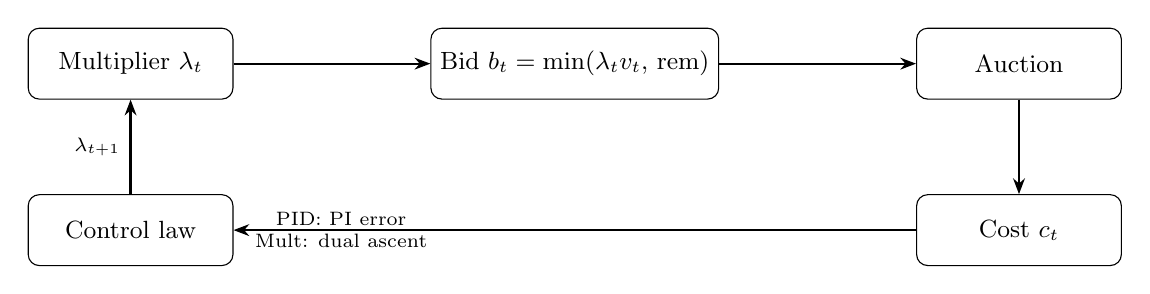
\begin{tikzpicture}[
  node distance=1.8cm and 2.5cm,
  block/.style={rectangle, draw, rounded corners, minimum width=2.6cm,
                minimum height=0.9cm, text centered, font=\small},
  arrow/.style={-{Stealth[length=2mm]}, thick},
]
  % Nodes
  \node[block] (mult)   {Multiplier $\lambda_t$};
  \node[block, right=of mult] (bid)    {Bid $b_t = \min(\lambda_t v_t,\,\text{rem})$};
  \node[block, right=of bid]  (auction){Auction};
  \node[block, below=1.2cm of auction] (cost)  {Cost $c_t$};
  \node[block, below=1.2cm of mult]  (ctrl)  {Control law};

  % Forward path
  \draw[arrow] (mult)    -- (bid);
  \draw[arrow] (bid)     -- (auction);
  \draw[arrow] (auction) -- (cost);
  \draw[arrow] (cost)    -- (ctrl);
  \draw[arrow] (ctrl)    -- node[left,font=\scriptsize]{$\lambda_{t+1}$} (mult);

  % Labels on control arrow
  \node[font=\scriptsize, align=center, right=0.15cm of ctrl]
    {PID: PI error\\Mult: dual ascent};
\end{tikzpicture}
\caption{Pacing feedback loop shared by both algorithms. The multiplier scales bids; auction outcomes feed back through the control law to update $\lambda$.}
\label{fig:pacing_loop}
\end{figure}

Budget tightness is parameterised as $\text{budget\_tightness} \times \mathbb{E}[v]\times T$, where $\mathbb{E}[v]=0.5$ for uniform marginals, matching the normalisation in Balseiro and Gur (2019). Note that $\eta$ throughout this paper denotes the affiliation parameter (Experiments~2--4); the dual step size above uses $\alpha_p$ to avoid notation collision.

\section{Experimental Design}

We design three experiments to study repeated sealed-bid auctions under varying valuations and learning strategies. In all experiments, $n$ bidders submit discrete bids $b_i\in[0,1]$ each round. A reserve price $r\ge 0$ may invalidate low bids below $r$. If no valid bid meets $r$, no sale occurs and the revenue is zero; otherwise, the highest valid bid wins, and any tie among top bids is broken at random. We compare first-price (winner pays her own bid) and second-price (winner pays the second-highest bid) formats. When multiple bids tie for the highest valid bid, our implementation selects a single winner uniformly at random among those tied. Each experiment allows multiple parameter configurations, as described in corresponding tables, and collects the outcome metrics listed below.

\paragraph{Experiment 1.} Here each bidder has a constant valuation $v_i=1.0$. This isolates how standard Q-learning responds to first- vs.\ second-price incentives when all players share the same private value of 1.0. Bidders maintain $Q$-values for pairs $(s,a)$, where $s$ can encode none, some, or all of the following: (i) the median of other bidders' previous-round bids and (ii) the previous winning bid. They update these $Q$-values either asynchronously (only the chosen action is updated per step) or synchronously (all actions are updated using counterfactual rewards). Table~\ref{tab:exp1params} summarizes the main parameters, including the learning rate $\alpha$, discount factor $\gamma$, exploration mode ($\varepsilon$-greedy or Boltzmann), number of bidders, reserve prices, and total training episodes. The combination of these factors tests how quickly bidders learn to match or shade their bids under the two payment rules.

\begin{table}[h]
\centering
\caption{Parameter settings for Experiment~1 (Constant Valuations).}
\label{tab:exp1params}
\begin{tabular}{l l}
\toprule
\textbf{Parameter} & \textbf{Possible Values}\\
\midrule
Number of bidders ($n$) & $\{2,4,6\}$\\
Reserve price ($r$) & $\{0.0,0.1,0.2,0.3,0.5\}$\\
Learning rate ($\alpha$) & e.g.\ $\{0.001,0.005,0.01,0.05,0.1\}$\\
Discount factor ($\gamma$) & e.g.\ $\{0.0,0.5,0.9,0.99\}$\\
Exploration & $\varepsilon$-greedy or Boltzmann\\
Q-update mode & Asynchronous or synchronous\\
State features & None / median-of-others / previous-winner\\
Number of episodes & e.g.\ $10^4$ or $10^5$\\
\bottomrule
\end{tabular}
\end{table}

\paragraph{Experiment 2.} Here bidders instead receive private signals $s_i\in[0,1]$, and their valuations become interdependent through an affiliation parameter $\eta\in[0,1]$ via $v_i=(1-0.5\,\eta)\,s_i + 0.5\,\eta\,\bigl(\tfrac{1}{n-1}\sum_{j\neq i}s_j\bigr)$. This lets $\eta=0$ represent purely private values and $\eta=1$ represent strong common-value elements, since each bidder’s valuation then weighs her own signal equally with that of her opponents. We again apply Q-learning with updates similar to Experiment\,1 but allow the current signal $s_i$ to appear in the bidder’s state. Table~\ref{tab:exp2params} highlights the key parameters, which still include choices for $\alpha$, $\gamma$, exploration strategy, number of bidders, reserve prices, and total episodes. By contrasting outcomes at different $\eta$ values, we observe how stronger affiliation (and thus more common-value features) affects revenue and convergence under first- vs.\ second-price rules.

\begin{table}[h]
\centering
\caption{Parameter settings for Experiment~2 (Affiliated Valuations + Q-learning).}
\label{tab:exp2params}
\begin{tabular}{l l}
\toprule
\textbf{Parameter} & \textbf{Possible Values}\\
\midrule
Number of bidders ($n$) & $\{2,4,6\}$\\
Reserve price ($r$) & $\{0.0,0.1,0.2,0.3\}$\\
Affiliation ($\eta$) & e.g.\ $\{0.0,0.25,0.5,0.75,1.0\}$\\
Learning rate ($\alpha$) & e.g.\ $\{0.001,0.005,0.01,0.05,0.1\}$\\
Discount factor ($\gamma$) & e.g.\ $\{0.0,0.5,0.9,0.99\}$\\
Exploration & $\varepsilon$-greedy or Boltzmann\\
Q-update mode & Asynchronous or synchronous\\
State features & e.g.\ $s_i,\,\text{median-of-others},\,\text{winner-bid}$\\
Number of episodes & e.g.\ $10^5$\\
\bottomrule
\end{tabular}
\end{table}

\paragraph{Experiment 3.} Here we preserve the signal-based, affiliated valuation model from Experiment\,2 but abandon Q-learning in favor of bandit-based methods. Each bidder treats possible bids as arms in either a standard multi-armed bandit or a linear contextual bandit (LinUCB), where the context could include the current signal plus optional median-of-others and winner-bid features. Exploration is controlled through an optimism bonus parameter $c$ rather than a learning rate or discount factor. A regularization parameter $\lambda$ may also be set to stabilize the bandit's linear estimates. Table~\ref{tab:exp3params} summarizes these parameters. This design highlights how structured bandit approaches might converge more efficiently than Q-learning, especially when valuations fluctuate with signals.

\begin{table}[H]
\centering
\caption{Parameter settings for Experiment~3 (Affiliated Valuations + Bandits).}
\label{tab:exp3params}
\begin{tabular}{l l}
\toprule
\textbf{Parameter} & \textbf{Possible Values}\\
\midrule
Number of bidders ($n$) & $\{2,4,6\}$\\
Reserve price ($r$) & $\{0.0,0.1,0.2,0.3,0.4,0.5\}$\\
Affiliation ($\eta$) & e.g.\ $\{0.0,0.25,0.5,0.75,1.0\}$\\
Bandit type & UCB or LinUCB\\
Exploration parameter ($c$) & e.g.\ $\{0.01,\dots,2.0\}$\\
Regularization ($\lambda$) & e.g.\ $\{0.1,1.0,5.0\}$\\
State features & e.g.\ $s_i,\,\text{median-of-others},\,\text{winner-bid}$\\
Number of rounds & e.g.\ $10^5$\\
\bottomrule
\end{tabular}
\end{table}

\subsection{Parameter Ranges in Experiments}
Table~\ref{tab:params} summarizes the parameters used across all experiments, their descriptions, and the ranges explored. A checkmark indicates that the parameter is applicable in a given experiment. 

\begin{table}[H]
\centering
\caption{Parameter Ranges and Their Usage Across Experiments}
\label{tab:params}
\begin{tabular}{l l l c c c}
\toprule
\textbf{Name} & \textbf{Description} & \textbf{Range} & \textbf{E1} & \textbf{E2} & \textbf{E3}\\
\midrule
$\alpha$ & Q-learning rate & $\{0.001,0.005,0.01,0.05,0.1\}$ & \checkmark & \checkmark & \\
$\gamma$ & Discount factor & $\{0.0,0.25,0.5,0.75,0.9,0.95,0.99\}$ & \checkmark & \checkmark & \\
$\varepsilon$ & E-greedy exploration prob & Typically decays from 1 to 0 & \checkmark & \checkmark & \\
Boltzmann & Softmax exploration & Weight factor over $Q$-values & \checkmark & \checkmark & \\
$c$ & Bandit exploration param & E.g.\ $[0.01,2.0]$ &  &  & \checkmark \\
$r$ & Reserve price & $\{0.0,0.1,0.2,0.3,0.4,0.5\}$ & \checkmark & \checkmark & \checkmark \\
$n$ & Number of bidders & $\{2,4,6\}$ or similar & \checkmark & \checkmark & \checkmark \\
$\eta$ & Affiliation parameter & $[0,1]$ &  & \checkmark & \checkmark \\
\textit{Episodes} & Total training rounds & E.g.\ $\{10{,}000, 50{,}000, 100{,}000\}$ & \checkmark & \checkmark & \checkmark \\
\textit{Sync/Async} & Q-learning modes & N/A (binary choice) & \checkmark & \checkmark & \\
\textit{Median/Winner} & State features & N/A (binary choice) & \checkmark & \checkmark & \checkmark\\
\bottomrule
\end{tabular}
\end{table}

\paragraph{Outcome Metrics.} Our outcome metrics are consistent across all three experiments. We measure the \emph{average revenue in later rounds}, typically by averaging the revenue over the final 1000 episodes, which reflects how well the auction performs after strategies have stabilized. We also determine the \emph{time to converge} as the earliest round after which the rolling-average revenue remains within $\pm 5\%$ of its final mean. We define \emph{seller regret} as $1 - (\text{observed revenue})$ per round to gauge how far earnings fall below the maximal payoff of 1. We compute a \emph{no-sale rate} by noting the fraction of rounds in which no valid bid exceeds the reserve. We track \emph{price volatility} by taking the sample standard deviation of winning bids in later rounds. Finally, we measure \emph{winner entropy} to see whether a particular bidder tends to dominate, calculating the Shannon entropy of the empirical distribution of winners. Table~\ref{tab:outcomes} provides a concise summary of these common metrics that allow systematic comparisons of convergence speed, bidding stability, and revenue performance across all experiments.

\begin{table}[h]
\centering
\caption{Outcome metrics used in all experiments.}
\label{tab:outcomes}
\begin{tabular}{l l}
\toprule
\textbf{Metric} & \textbf{Description}\\
\midrule
Average revenue (later rounds) & Mean revenue in the final 1000 rounds \\
Time to converge & Round at which revenue stays in a $\pm 5\%$ band \\
Seller regret & $1-\text{(realized revenue per round)}$\\
No-sale rate & Fraction of rounds with all bids below $r$\\
Price volatility & Standard deviation of winning bids in later rounds \\
Winner entropy & Shannon entropy of bidder identity distribution \\
\bottomrule
\end{tabular}
\end{table}

\section{Statistical Inference}
\label{sec:inference}

\subsection{Factorial Design Framework}

We employ $2^k$ factorial designs to systematically explore the parameter space of each experiment. Every factor is coded as $x_i \in \{-1, +1\}$\footnote{Effects coding ($\{-1, +1\}$) differs from indicator (dummy) coding ($\{0, 1\}$). Under effects coding, the intercept $\beta_0$ equals the grand mean of all observations, and each $\beta_j$ measures the deviation of a factor level from that grand mean. This yields orthogonal contrasts in balanced designs, so that main effects and interactions are estimated independently. Indicator coding would confound the intercept with the reference level and introduce correlations between estimators in factorial models.}, representing its low and high levels respectively. This coding ensures orthogonality: factor estimates are uncorrelated, and the design provides balanced variance across the entire experimental region. The balanced structure guarantees that each main effect and two-way interaction can be estimated independently of all others, enabling clean attribution of outcome variation to specific factors.

Experiment~1 uses a $2^{11-1}$ Resolution~V half-fraction with 11 factors and 1{,}024 design cells, replicated twice for 2{,}048 observations. Experiment~2 uses a $3 \times 2^3$ mixed-level design with 4 factors (3 binary plus the three-level affiliation parameter $\eta$) and 24 cells, replicated twice for 48 observations. Experiment~3 uses a $3 \times 2^7$ mixed-level design with 8 factors (7 binary plus $\eta$) and 384 cells, replicated twice for 768 observations. Experiment~4 uses a $2^3$ full factorial with 3 factors and 8 cells, each replicated across 50 independent seeds for 400 observations. Replication in all experiments enables pure error estimation and lack-of-fit testing.

\subsection{Estimation}

For each response variable $Y$ (e.g., average revenue, seller regret, convergence time), we fit a linear model with main effects and all two-way interactions via ordinary least squares (OLS):
\begin{align}
  Y_i = \beta_0 + \sum_{j=1}^{k} \beta_j\, x_{ji} + \sum_{1 \le j < l \le k} \beta_{jl}\, x_{ji}\, x_{li} + \varepsilon_i,
  \label{eq:ols}
\end{align}
where $x_{ji} \in \{-1, +1\}$ is the coded level of factor $j$ in observation $i$, $\beta_j$ represents the main effect of factor $j$, and $\beta_{jl}$ captures the two-way interaction between factors $j$ and $l$. Under the coded parameterisation, $\beta_j$ equals half the change in mean response when factor $j$ moves from its low to its high level, holding all other factors at their centre values. Similarly, $\beta_{jl}$ equals half the difference in the effect of factor $j$ between the two levels of factor $l$.

We use Type~III ANOVA decomposition to assess the marginal contribution of each term, testing each coefficient against the null $H_0\!: \beta = 0$ via the $t$-statistic $\hat{\beta}/\text{SE}(\hat{\beta})$. Model adequacy is validated by comparing OLS $R^2$ to a gradient-boosted machine (LightGBM) $R^2$ trained with five-fold cross-validation: if the gap is less than 0.05, the linear model with two-way interactions captures most of the signal without requiring higher-order terms or nonlinear transformations.

\subsection{Fractional Factorial Designs and Aliasing}

Experiment~1 uses a fractional factorial design to reduce experimental burden. The key trade-off is aliasing: some higher-order interactions become confounded with lower-order terms. Experiments~2 and~3 use mixed-level designs (combining the three-level $\eta$ factor with binary factors), and Experiment~4 uses a full $2^3$ factorial, so aliasing is not a concern for these experiments.

\subsubsection{Resolution~V (Experiment~1)}

In a Resolution~V\footnote{In a Resolution~$R$ design, no $p$-factor interaction is aliased with any interaction of fewer than $R - p$ factors. Resolution~V therefore guarantees that main effects are free of two-way interaction bias and two-way interactions are free of other two-way interaction bias.} design, no main effect is aliased with any interaction of fewer than four factors, and no two-way interaction is aliased with any interaction of fewer than three factors. This ensures that all main effects and two-way interactions are estimable without bias from three-way terms, which are assumed negligible under effect sparsity.

The assumption underlying the fractional design is \emph{effect sparsity}: most variation in the response is explained by main effects and two-way interactions, with three-way and higher interactions contributing negligibly. We validate this assumption using LASSO variable selection and nonparametric model comparison.

\subsection{Robustness Checks}

\subsubsection{Inference Corrections}

We compute HC3 robust standard errors (MacKinnon and White, 1985) to account for non-constant error variance across the design space. Comparing OLS standard errors to HC3 robust standard errors, we verify that significance claims hold under heteroscedasticity. The fraction of effects changing significance status under HC3 ranges from 0\% (Experiment~4) to 6.7\% (Experiment~1); per-experiment details appear in Sections~\ref{sec:exp1_robustness} through~\ref{sec:exp4_robustness}.

With $k$ main effects, $\binom{k}{2}$ two-way interactions, and $m$ response variables, each experiment involves many simultaneous hypothesis tests. We apply Holm--Bonferroni sequential correction (Holm, 1979) to control the family-wise error rate at $\alpha = 0.05$. Key findings, including the auction type main effect and the auction type $\times$ exploration interaction, survive this stringent correction across all responses.

For the top~10 effects by absolute $t$-statistic in each response, we compute Rademacher wild bootstrap $p$-values (1{,}000 iterations) to validate inference under minimal distributional assumptions. Bootstrap $p$-values align closely with HC3 asymptotic $p$-values (differences below 0.01), confirming robustness.

We fit quantile regressions at the 10th, 25th, 50th, 75th, and 90th percentiles of each response to assess whether factor effects are uniform across the outcome distribution or concentrated in the tails. An effect that is large at extreme quantiles but small at the median indicates that the factor primarily influences worst-case or best-case configurations rather than the typical outcome. This complements the OLS analysis, which estimates effects at the conditional mean.

\subsubsection{Model Adequacy}

With two replicates per cell, we decompose the residual sum of squares into pure error (within-cell variation) and lack of fit (deviation of cell means from model predictions). The $F$-test $\text{MS}_{\text{LOF}} / \text{MS}_{\text{PE}}$ assesses whether the linear model with two-way interactions adequately fits the data. Per-experiment lack-of-fit results are reported in Sections~\ref{sec:exp1_robustness} through~\ref{sec:exp4_robustness}.

We compute leave-one-out cross-validated $R^2$ using the PRESS statistic:
\begin{align}
  \text{PRESS} = \sum_{i=1}^{n} \left( \frac{e_i}{1 - h_{ii}} \right)^{\!2}, \qquad
  \text{Pred-}R^2 = 1 - \frac{\text{PRESS}}{\text{SS}_{\text{Total}}},
  \label{eq:press}
\end{align}
where $e_i$ is the $i$-th ordinary residual and $h_{ii}$ is the $i$-th diagonal element of the hat matrix. A gap between $R^2$ and Pred-$R^2$ smaller than 0.10 indicates minimal overfitting. Predicted $R^2$ and PRESS gaps vary across experiments and are reported in each experiment's model adequacy table (Tables~\ref{tab:exp1_adequacy}--\ref{tab:exp4_adequacy}).

Gradient-boosted machines (LightGBM, 200 trees, maximum depth~4) are fit using five-fold cross-validation to establish a nonparametric upper bound on achievable $R^2$. If OLS $R^2$ is within 0.05 of LightGBM $R^2$, we conclude that the linear model with two-way interactions captures most of the signal and that higher-order or nonlinear terms contribute negligibly. In all experiments, OLS $R^2$ meets or exceeds LightGBM cross-validated $R^2$, confirming that the parametric model is well suited to the balanced factorial structure (see per-experiment diagnostics in Tables~\ref{tab:exp1_adequacy}--\ref{tab:exp4_adequacy}).

\subsubsection{Variable Selection and Power}

We fit five-fold cross-validated LASSO models with regularisation parameter $\lambda$ chosen to minimise mean squared error. Surviving variables are compared to OLS significance: in all experiments, LASSO retains auction type and number of bidders, corroborating OLS effect selection. Heredity is verified by checking that no interaction survives whose parent main effects were dropped.

We compute minimum detectable effects (MDE) at 80\% power and $\alpha = 0.05$ for balanced $2^k$ designs:
\begin{align}
  \text{MDE}_{\text{main}} = \bigl(t_{\text{crit}} + t_{0.80}\bigr) \times \frac{\hat{\sigma}}{\sqrt{n}},
  \label{eq:mde}
\end{align}
where $t_{\text{crit}}$ is the critical value at $\alpha/2$, $t_{0.80}$ is the 80th percentile of the $t$-distribution, $\hat{\sigma}$ is the estimated residual standard deviation, and $n$ is the total number of observations. MDEs range from 2--5\% of the mean response, indicating that the designs have sufficient power to detect practically meaningful effects.

\subsection{Diagnostic Visualisations}

Four types of diagnostic plots accompany each response variable. Pareto charts rank effects by absolute $t$-statistic in descending order, with effects surpassing the critical threshold $t_{\alpha/2,\,\text{df}}$ shown in red, providing a visual hierarchy of effect importance. Main effects plots display the mean response at the low ($-1$) and high ($+1$) levels of each factor; steeper slopes correspond to larger $|\beta_j|$ values. Interaction plots show the mean response across the four combinations $(x_j, x_l) \in \{(-1,-1), (-1,+1), (+1,-1), (+1,+1)\}$ for the top six interactions by $|t|$-statistic; non-parallel lines indicate that the effect of one factor depends on the level of another. Half-normal probability plots display $|\hat{\beta}_j|$ against expected order statistics from a half-normal distribution, separating active effects (large departures from the reference line) from noise (points following the line). Residual diagnostics include quantile--quantile plots assessing normality and residuals-versus-fitted plots checking for heteroscedasticity and nonlinearity.

\subsection{Reporting}

All results report OLS coefficients with standard errors. Effect sizes are interpreted as practical significance (magnitude relative to mean response) in addition to statistical significance ($p$-value threshold). Each experiment's results section includes a model adequacy table (Tables~\ref{tab:exp1_adequacy}--\ref{tab:exp4_adequacy}) reporting $R^2$, Pred-$R^2$, LightGBM $R^2$, and lack-of-fit $p$-value, and an inference robustness table (Tables~\ref{tab:exp1_inference}--\ref{tab:exp4_inference}) reporting HC3 flips, Holm--Bonferroni survivors, and Benjamini--Hochberg survivors. All effects reported as statistically significant in the results sections survive Benjamini--Hochberg correction.

\section{Results: Experiment 1}

The summary statistics confirm that the experimental design randomly allocated parameters across treatment conditions: none of the main covariates (e.g., learning rate $\alpha$, discount factor $\gamma$, or initialization strategy) shows correlation with \texttt{auction\_type\_code}. Despite true valuations of 1 for all bidders, the final 1000-episode average revenues (\texttt{avg\_rev\_last\_1000}) span a broad range (0.3 to 1.0), highlighting substantial variability stemming from different learning and auction interactions.

\subsection*{Reveues and Seller Regret}

\paragraph{First-Price Auctions Reduce Revenues.}
DoubleML estimates reveal that switching to a first-price format (\texttt{auction\_type\_code} $=1$) significantly lowers final revenue on average by about 0.0945 ($p<0.0001$) and raises the seller’s regret on average by 0.0651 ($p<0.0001$). Other outcomes, including convergence time and price volatility, remain statistically insignificant. The no-sale rate trends modestly higher under first-price but does not reach conventional significance ($p \approx 0.082$). 

\input{tables/exp1_ate}

\paragraph{Fewer Bidders and Very High Discount Factors Worsen Collusion.}
Conditional average treatment effect (CATE) results indicate that having more bidders offsets part of the revenue penalty from first-price auctions: as \(\texttt{n\_bidders}\) increases, the negative effect on final revenue shrinks. In contrast, higher \(\gamma\) slightly exacerbates the first-price reduction, presumably because agents with a stronger focus on future returns adopt more conservative near-term bidding. 

\begin{figure}[H]
\centering
\begin{minipage}{0.45\linewidth}
  \centering
  \includegraphics[width=\textwidth]{figures/e1_reg_bidder.png}
\end{minipage}
\hfill
\begin{minipage}{0.45\linewidth}
  \centering
  \includegraphics[width=\textwidth]{figures/e1_rev_bidder.png}
\end{minipage}
\\[1em]
\begin{minipage}{0.45\linewidth}
  \centering
  \includegraphics[width=\textwidth]{figures/e1_reg_gamma.png}
\end{minipage}
\hfill
\begin{minipage}{0.45\linewidth}
  \centering
  \includegraphics[width=\textwidth]{figures/e1_rev_gamma.png}
\end{minipage}
\caption{Illustrative CATE partial-dependence plots in a 2$\times$2 grid.}
\label{fig:cate_2x2}
\end{figure}

\paragraph{Exploration and Update Mode.}
Group-average treatment effect (GATE) comparisons indicate that $\varepsilon$-greedy exploration intensifies first-price losses (a revenue drop of $-0.1420$) relative to Boltzmann exploration ($-0.0339$), a substantial difference ($p<0.0001$) that highlights how a more controlled and probabilistic (Boltzmann) approach mitigates aggressive underbidding. Likewise, asynchronous Q-updates increase the magnitude of first-price losses ($-0.1161$) compared to synchronous updates ($-0.0683$), a significant difference ($p=0.0010$). In other words, \emph{synchronous} Q-learning dampens the detrimental impact of first-price auctions, likely by maintaining more uniform knowledge updates across all possible actions and bidders.

\input{tables/exp1_gate}

\subsection{Price Volatility and No-Sale}

Beyond the highly significant results for \textit{avg\_rev\_last\_1000} (revenue) and \textit{avg\_regret\_of\_seller}, two other findings merit attention:

\paragraph{Price Volatility.}
Although the average treatment effect (ATE) on \(\texttt{price\_volatility}\) is not significant (\(p=0.2540\)), the group-average treatment effect (GATE) analysis reveals that volatility outcomes depend significantly on both \(\texttt{exploration\_code}\) (\(\Delta=0.0112\), \(t=2.962\), \(p=0.0031\)) and \(\texttt{asynchronous\_code}\) (\(\Delta=0.0089\), \(t=2.633\), \(p=0.0085\)). In other words, while first-price auctions do not generally raise volatility on average, they \emph{do} if the agents rely on $\varepsilon$-greedy exploration or asynchronous Q-learning updates. Further, increasing the number of bidders modestly increases the price volatility under first-price auctions. The CATE turns slightly positive with higher bidders.  

\begin{figure}[H]
\centering
\includegraphics[width=0.5\textwidth]{figures/e1_vol_bidder.png}
\caption{CATE partial-dependence plot for number of bidders.}
\label{fig:volatility_vs_bidders}
\end{figure}

\paragraph{No-Sale Rate.}
The estimated ATE on \(\texttt{no\_sale\_rate}\) yields a \(p\)-value near \(0.082\), suggesting a slight upward trend under first-price auctions. Although this does not meet the strict 5\% threshold, it is sufficiently close to underscore a modest likelihood that first-price auctions may increase the fraction of no-bid rounds (where no agents' bid exceeds the reserve price).

\subsection{Summary}

Overall, first-price auctions were associated with substantially lower final revenues and noticeably higher seller regret. These effects were buffered by having a larger pool of bidders, but were intensified by higher discount factors. Exploration strategy and update mode both played significant roles in shaping outcomes: synchronous updates and Boltzmann exploration helped curtail the losses under first-price, whereas asynchronous updates and $\varepsilon$-greedy exploration amplified them. Although price volatility did not increase under first-price on average, it did when agents used asynchronous updating or $\varepsilon$-greedy exploration. It also did when there were a larger number of bidders, pushing against the view that more bidders are always better. Finally, while there was only a borderline effect on the fraction of no-sale episodes, the data suggest a slight tendency toward more such episodes under first-price auctions. These results are fairly unambiguous from a seller's point of view: first price auctions do not fare well when algorithms learn. 

\section{Experiment II: Q-Learning under Affiliated Valuations}

\begin{figure}[H]
  \centering
  \includegraphics[width=\textwidth]{figures/e2_trace}
  \caption{Representative learning trajectory for a single trial of Experiment~2 (first-price auction, $\eta = 0.5$, 2~bidders, 10{,}000 episodes). Top: rolling-mean revenue converging near the BNE prediction. Bottom: raw per-episode revenue in the final 2{,}000 episodes, illustrating residual variance around the equilibrium level.}
  \label{fig:e2_trace}
\end{figure}

Experiment~2 generalises the Q-learning framework to affiliated valuations by introducing the affiliation parameter $\eta \in \{0, 1\}$. The design is a $2^{11-1}$ Resolution~V half-fraction with 11 factors and 2{,}048 observations. The primary question is whether valuation interdependence, ranging from purely private values ($\eta = 0$) to near-common values ($\eta = 1$), alters the relative performance of first-price and second-price auctions under algorithmic bidding.

\subsection{Revenue and Seller Regret}

First-price auctions again significantly reduce revenue and increase seller regret. Table~\ref{tab:exp2_ranked_rev} confirms that auction type dominates the effect hierarchy, followed by exploration strategy and the number of bidders, replicating the factor ordering from Experiment~1. The main effects plots (Figures~\ref{fig:e2_main_rev} and~\ref{fig:e2_main_reg}) show that first-price auctions ($+1$) consistently underperform second-price auctions ($-1$) across both revenue and regret.

\input{tables/exp2_ranked_rev}

\begin{figure}[H]
  \centering
  \includegraphics[width=0.7\textwidth]{figures/e2_main_rev}
  \caption{Experiment~2: Main effects plot for average revenue. First-price auctions reduce revenue across all factor configurations.}
  \label{fig:e2_main_rev}
\end{figure}

\input{tables/exp2_ranked_reg}

\begin{figure}[H]
  \centering
  \includegraphics[width=0.7\textwidth]{figures/e2_main_reg}
  \caption{Experiment~2: Main effects plot for seller regret.}
  \label{fig:e2_main_reg}
\end{figure}

The affiliation parameter $\eta$ shows no statistically significant effect on any primary outcome. Despite spanning the full range from independent private values to near-common values, $\eta$ does not materially alter the relative performance of auction formats. This null result is striking: whether valuations are purely private or highly correlated, learning agents display similar bidding patterns, and the auction mechanism ($\text{first-price}$ vs.\ $\text{second-price}$) overshadows valuation interdependence in shaping long-run outcomes.

Exploration strategy remains pivotal. As in Experiment~1, Boltzmann exploration dramatically reduces the first-price shortfall, while $\varepsilon$-greedy agents intensify the negative effects. The number of bidders continues to moderate the auction type effect, with more bidders dampening the revenue penalty from first-price auctions. The interaction plot (Figure~\ref{fig:e2_int_rev}) displays these moderating relationships, showing how auction format interacts with exploration and competitive pressure.

\begin{figure}[H]
  \centering
  \includegraphics[width=0.7\textwidth]{figures/e2_int_rev}
  \caption{Experiment~2: Interaction plot for average revenue. The auction type $\times$ exploration and auction type $\times$ number of bidders interactions are among the strongest two-way effects.}
  \label{fig:e2_int_rev}
\end{figure}

\subsection{Price Volatility}

Unlike Experiment~1, where auction type had minimal effect on volatility, first-price auctions now significantly raise price volatility under affiliated valuations. Table~\ref{tab:exp2_ranked_vol} shows auction type among the significant effects for volatility. The main effects plot (Figure~\ref{fig:e2_main_vol}) confirms the directional increase. Initialisation strategy also contributes: starting Q-values at zeros rather than random values slightly amplifies the first-price volatility gap.

\input{tables/exp2_ranked_vol}

\begin{figure}[H]
  \centering
  \includegraphics[width=0.7\textwidth]{figures/e2_main_vol}
  \caption{Experiment~2: Main effects plot for price volatility.}
  \label{fig:e2_main_vol}
\end{figure}

\subsection{Model Fit and Significant Effects}

\input{tables/exp2_model_fit}

\input{tables/exp2_significant}

\subsection{Summary}

Even under affiliated valuations, first-price auctions yield significantly lower revenue, greater seller regret, and higher price volatility than second-price auctions. The affiliation parameter $\eta$ has no significant impact on any primary outcome, implying that the private-versus-common value distinction is irrelevant to the collusion dynamics studied here. Increasing the number of bidders alleviates some first-price drawbacks but does not eliminate them, and exploration strategy remains the key moderator. These results reinforce the conclusion from Experiment~1 that first-price auctions perform poorly under algorithmic bidding, and demonstrate that this finding is robust to the introduction of valuation interdependence.

\section{Experiment III: Contextual Bandits}

\begin{figure}[H]
  \centering
  \includegraphics[width=\textwidth]{figures/e3_trace}
  \caption{Representative learning trajectory for a single trial of Experiment~3 (LinUCB, first-price auction, $\eta = 0.5$, 2~bidders, 5{,}000 rounds). Top: rolling-mean revenue with BNE benchmark. Middle: bid versus signal in the final 1{,}000 rounds, overlaid with the BNE bid function. Bottom: cumulative average reward per bidder.}
  \label{fig:e3_trace}
\end{figure}

Experiment~3 replaces Q-learning with LinUCB contextual bandits, testing whether a more sophisticated exploration mechanism improves seller outcomes. The design is a $2^8$ full factorial with 8 factors and 512 observations. The outcome range widens substantially relative to Experiment~2: certain runs converge to near-zero revenue or universal no-sales, while others perform comparably to Q-learning. Mean revenue drops and mean seller regret rises, with more polarised extremes of volatility, winner entropy, and no-sale rates. This highlights how contextual exploration can magnify variability in auction outcomes rather than reliably benefiting the seller; a finding that challenges the common criticism of Q-learning studies, which argues that firms would adopt more efficient exploration algorithms to improve outcomes.

\subsection{Revenue and Seller Regret}

Auction type remains the dominant factor, with the largest absolute $t$-statistic ($|t| \approx 12$) for both revenue and regret. Table~\ref{tab:exp3_ranked_rev} shows that auction type is followed by number of bidders and the exploration parameter $c$. First-price auctions yield substantially lower final revenue and higher seller regret, as the main effects plots (Figures~\ref{fig:e3_main_rev} and~\ref{fig:e3_main_reg}) confirm.

\input{tables/exp3_ranked_rev}

\begin{figure}[H]
  \centering
  \includegraphics[width=0.7\textwidth]{figures/e3_main_rev}
  \caption{Experiment~3: Main effects plot for average revenue. First-price auctions produce markedly lower revenue than second-price.}
  \label{fig:e3_main_rev}
\end{figure}

\input{tables/exp3_ranked_reg}

\begin{figure}[H]
  \centering
  \includegraphics[width=0.7\textwidth]{figures/e3_main_reg}
  \caption{Experiment~3: Main effects plot for seller regret. The mirror image of the revenue pattern.}
  \label{fig:e3_main_reg}
\end{figure}

The affiliation parameter $\eta$ again shows no statistically significant effect on any primary outcome, consistent with Experiment~2. Even in this bandit-based setting, increasing affiliation does not meaningfully change the outcome gaps between auction formats.

Contrary to Q-learning experiments, more bidders \emph{worsen} first-price performance under LinUCB. Increased competition does not mitigate strategic underbidding; instead, it amplifies it, leading to worse revenue and regret as the number of bidders rises. This reversal from Experiments~1 and~2 suggests that optimism-based exploration interacts with competitive pressure differently than $\varepsilon$-greedy or Boltzmann exploration.

The exploration parameter $c$ has a significant negative effect on revenue, indicating that higher exploration incentives reduce final revenues. This challenges the assumption that efficient exploration benefits sellers: LinUCB's optimism-based mechanism may reinforce risk-averse bidding by inflating uncertainty estimates around aggressive actions that rarely win. The interaction plot (Figure~\ref{fig:e3_int_rev}) shows these moderating effects and the departures from additivity among the top factorial interactions.

\begin{figure}[H]
  \centering
  \includegraphics[width=0.7\textwidth]{figures/e3_int_rev}
  \caption{Experiment~3: Interaction plot for average revenue under LinUCB. Non-parallel lines indicate factor interdependencies, including the bidder-count reversal.}
  \label{fig:e3_int_rev}
\end{figure}

\subsection{Price Volatility}

Under LinUCB bandits, price volatility is \emph{lower} in first-price auctions, the opposite direction from Experiment~2. Table~\ref{tab:exp3_ranked_vol} and the main effects plot (Figure~\ref{fig:e3_main_vol}) confirm this reversal. The result suggests that first-price auctions under LinUCB produce more uniform (though lower) winning bids, as agents converge to stable but suboptimal bid-shading equilibria. Reserve prices also show a significant negative effect on volatility, stabilising winning bids by disqualifying extreme low bids.

\input{tables/exp3_ranked_vol}

\begin{figure}[H]
  \centering
  \includegraphics[width=0.7\textwidth]{figures/e3_main_vol}
  \caption{Experiment~3: Main effects plot for price volatility.}
  \label{fig:e3_main_vol}
\end{figure}

\subsection{Model Fit and Significant Effects}

\input{tables/exp3_model_fit}

\input{tables/exp3_significant}

\subsection{Summary}

Replacing Q-learning with LinUCB contextual bandits amplifies variability in auction outcomes and does not improve seller welfare. First-price auctions produce substantially lower revenue and higher regret under bandits than under Q-learning, with the revenue gap widening dramatically. The exploration parameter $c$ reduces rather than improves revenue, and more bidders worsen first-price performance; both reversals from Q-learning experiments. These findings demonstrate that algorithmic sophistication does not inherently mitigate the disadvantages of first-price auctions and can exacerbate negative outcomes when the exploration mechanism reinforces conservative bidding.


\section{Conclusion}

A consistent finding across all three experiments is that first-price auctions systematically yield lower revenue and higher seller regret than their second-price counterparts. This pattern persists regardless of whether bidders have constant valuations, affiliated valuations, or whether the learning agents are Q-learners or LinUCB bandits. The recurring shortfall in revenue underscores how first-price mechanisms can incentivize overly conservative (or collusive) bidding strategies among learning agents.

A greater number of bidders improves performance in first-price auctions when agents rely on Q-learning, reducing the revenue gap relative to second-price. However, the opposite emerges with LinUCB bandits, where more participants appear to amplify underbidding. This divergence suggests that standard economic intuition—where increased competition drives up bids—may be upended by different algorithmic forms of learning and exploration.

The Q-learning experiments reveal that a high discount factor intensifies the first-price underperformance. When agents place greater weight on future outcomes, they seem more motivated to shade bids aggressively in the near term, possibly hoping for improved payoffs over the long run. By contrast, second-price auctions do not appear as sensitive to this temporal consideration, maintaining relatively stable performance across different discount-factor regimes.


The manner in which agents explore significantly alters the extent of first-price losses. Boltzmann exploration, which selects actions with probabilities weighted by current value estimates, tends to mitigate underbidding. In contrast, \(\varepsilon\)-greedy exploration—where agents pick the best-known action or otherwise randomize uniformly—reinforces strategic conservatism in first-price auctions and leads to lower overall revenue.

In Q-learning, synchronous updates that adjust the action-value function for all actions—rather than solely the chosen one—help curb the detrimental effects of first-price. This more thorough learning process appears to limit persistent miscalibrations, ensuring that alternative bidding strategies are not neglected. Asynchronous updates, by updating only the chosen bid each round, permit entrenched underbidding equilibria to emerge more readily.

Switching from Q-learning to a bandit framework (particularly LinUCB) was expected to offer more “sophisticated” or “efficient” exploration. Yet, our results show that bandit-based bidders can produce more polarized outcomes, including extremely low-revenue equilibria and frequent no-sales. Rather than improving overall seller payoffs, this more advanced contextual approach may exacerbate the strategic gap between first- and second-price auctions.

Though we introduced affiliated valuations via the parameter \(\eta\), it did not significantly alter the core first- versus second-price revenue gap in any of the experiments. Whether values were purely private (\(\eta=0\)) or close to common (\(\eta=1\)), learning agents displayed similar bidding patterns across auction formats. In practice, this implies that the mechanism choice may overshadow the importance of valuation interdependence in shaping long-run auction outcomes under learning.

Reserve prices show limited direct impact on final revenue but can reduce bidding volatility under first-price auctions. By disqualifying very low bids, reserves effectively raise the floor of competition, discouraging extreme shading and limiting the range of payoffs. Nonetheless, such price floors cannot by themselves resolve the fundamental underperformance of first-price formats revealed in these experiments.

Taken together, these findings point to a central conclusion: when bidders are learning autonomously, second-price auctions tend to outperform first-price auctions across a wide variety of settings and parameters. Even so, the nature of the learning algorithm—Q-learning versus contextual bandits—strongly influences the severity and form of underbidding behaviors. From a practical standpoint, designers seeking robust revenue outcomes in algorithmic bidding environments may wish to favor second-price mechanisms or employ additional tools (e.g., carefully tuned reserves, offer information so that synchronous updating can take place) that limit first-price collusion.

\paragraph{Budget Constraints as a Structural Moderator.}
Experiment~4 reveals a fourth moderating force: spending constraints. Budget-constrained pacing agents converge substantially faster than unconstrained Q-learners or LinUCB bandits---median convergence occurs around 1{,}000 rounds versus 22{,}730 rounds for the bandit experiment---suggesting that the hard budget cap forces early settlement into stable bidding patterns. This convergence acceleration parallels the role of high exploration parameters in earlier experiments: both introduce a form of forced commitment that prevents indefinite experimentation. The dominant factor across all nine response variables is \emph{budget tightness}: tighter budgets raise auction revenue, mirroring optimal auction theory's prediction that binding capacity constraints increase allocative pressure (Myerson 1981). The algorithm choice (PID vs.\ multiplicative) is the second strongest factor, with PID generating approximately 35\% higher revenue overall. Crucially, the \emph{algorithm $\times$ budget tightness} interaction reveals that the PID advantage is largest precisely when budgets are tight---PID's integral correction allows finer pacing control under binding constraints, whereas the multiplicative algorithm's dual variable can oscillate near the budget boundary. This dynamic is consistent with the tractability results in Conitzer et al.\ (2022): first-price pacing equilibria (FPPE) are polynomial-time computable, and PID converges toward them more reliably. Aggressiveness in pacing plays a structurally analogous role to exploration in Q-learning: higher aggressiveness raises revenue in first-price auctions by preventing excessive bid shading, the same mechanism by which Boltzmann exploration reduces collusion in Experiments~1 and~2. Taken together, these results extend the core conclusion: budget constraints do not eliminate the first-price underperformance, but they substantially attenuate it through forced pacing discipline---a finding with direct implications for programmatic advertising markets where budget-constrained DSPs participate in repeated first-price auctions.
\appendix
\section{References}

\begin{enumerate}
    \item Abada, Ibrahim, Xavier Lambin, and Nikolay Tchakarov. 2022. “Collusion by Mistake: Does Algorithmic Sophistication Drive Supra-Competitive Profits?” \textit{SSRN Electronic Journal}. \url{https://doi.org/10.2139/ssrn.4099361}.
    
    \item Asker, John, Chaim Fershtman, and Ariel Pakes. 2022. “Artificial Intelligence, Algorithm Design, and Pricing.” \textit{AEA Papers and Proceedings} 112 (May): 452–56. \url{https://doi.org/10.1257/pandp.20221059}.
    
    \item Assad, Stephanie, Robert Clark, Daniel Ershov, and Lei Xu. 2020. “Algorithmic Pricing and Competition: Empirical Evidence from the German Retail Gasoline Market.” \textit{SSRN Electronic Journal}. \url{https://doi.org/10.2139/ssrn.3682021}.
    
    \item Athey, Susan, and Guido Imbens. 2016. “The Econometrics of Randomized Experiments.” \textit{arXiv}. \url{http://arxiv.org/abs/1607.00698}.
    
    \item Banchio, Martino, and Andrzej Skrzypacz. 2022. “Artificial Intelligence and Auction Design.” In \textit{Proceedings of the 23rd ACM Conference on Economics and Computation}, 30–31. Boulder CO USA: ACM. \url{https://doi.org/10.1145/3490486.3538244}.
    
    \item Banchio, Martino, and Giacomo Mantegazza. 2022. “Adaptive Algorithms and Collusion via Coupling.” \textit{arXiv}. \url{http://arxiv.org/abs/2202.05946}.
    
    \item Bandyopadhyay, Subhajyoti, Jackie Rees, and John M. Barron. 2008. “Reverse Auctions with Multiple Reinforcement Learning Agents.” \textit{Decision Sciences} 39 (1): 33–63. \url{https://doi.org/10.1111/j.1540-5915.2008.00181.x}.
        
    \item Calvano, Emilio, Giacomo Calzolari, Vincenzo Denicolò, and Sergio Pastorello. 2020. “Artificial Intelligence, Algorithmic Pricing, and Collusion.” \textit{American Economic Review} 110 (10): 3267–97. \url{https://doi.org/10.1257/aer.20190623}.
            
    \item Freedman, David A. 2008a. “On Regression Adjustments in Experiments with Several Treatments.” \textit{The Annals of Applied Statistics} 2 (1). \url{https://doi.org/10.1214/07-AOAS143}.
    
    \item Freedman, David A. 2008b. “On Regression Adjustments in Experiments with Several Treatments.” \textit{The Annals of Applied Statistics} 2 (1). \url{https://doi.org/10.1214/07-AOAS143}.
    
    \item Klein, Timo. 2021. “Autonomous Algorithmic Collusion: Q‐learning under Sequential Pricing.” \textit{The RAND Journal of Economics} 52 (3): 538–58. \url{https://doi.org/10.1111/1756-2171.12383}.
        
    \item Lin, Winston. 2013. “Agnostic Notes on Regression Adjustments to Experimental Data: Reexamining Freedman’s Critique.” \textit{The Annals of Applied Statistics} 7 (1). \url{https://doi.org/10.1214/12-AOAS583}.
                
\end{enumerate}

\newpage
\section{Appendix: Experiment 1 Results}

\subsection{Summary Statistics}
\begin{table}[H]
\centering
\caption{Summary Statistics for Experiment 1}
\label{tab:summary_statistics_exp1}
\small
\begin{tabular}{lrrrr}
\toprule
\textbf{Variable} & \textbf{Mean} & \textbf{Std} & \textbf{Min} & \textbf{Max} \\
\midrule
Learning rate ($\alpha$) & 0.033 & 0.036 & 0.001 & 0.100 \\
Discount factor ($\gamma$) & 0.615 & 0.356 & 0.000 & 0.990 \\
Update mode (async) & 0.500 & 0.501 & 0.000 & 1.000 \\
Number of bidders & 3.960 & 1.689 & 2.000 & 6.000 \\
Median opponent bid (state) & 0.498 & 0.501 & 0.000 & 1.000 \\
Winner bid (state) & 0.512 & 0.500 & 0.000 & 1.000 \\
Reserve price & 0.246 & 0.171 & 0.000 & 0.500 \\
Boltzmann temperature & 0.912 & 0.714 & 0.100 & 2.000 \\
Training episodes & 54{,}695 & 25{,}792 & 10{,}188 & 99{,}905 \\
Initialisation (zeros) & 0.514 & 0.500 & 0.000 & 1.000 \\
Exploration ($\varepsilon$-greedy) & 0.474 & 0.500 & 0.000 & 1.000 \\
Auction format (first-price) & 0.488 & 0.500 & 0.000 & 1.000 \\
\midrule
Average revenue & 0.844 & 0.127 & 0.300 & 1.000 \\
Convergence time & 0.320 & 0.380 & 0.000 & 0.954 \\
Seller regret & 0.225 & 0.135 & 0.051 & 0.659 \\
\bottomrule
\end{tabular}
\par\smallskip\footnotesize
Factor parameters (above the line) describe the experimental design; response variables (below) are measured outcomes.
\end{table}

\section{Appendix: Experiment 2 Results}

\subsection{Summary Statistics}
\begin{table}[H]
\centering
\caption{Summary Statistics for Experiment 2}
\label{tab:summary_statistics_exp2}
\small
\setlength{\tabcolsep}{3pt}
\begin{tabular}{lrrrrrrr}
\toprule
\textbf{Variable} & \textbf{Mean} & \textbf{Std} & \textbf{Min} & \textbf{25\%} & \textbf{50\%} & \textbf{75\%} & \textbf{Max} \\
\midrule
\texttt{eta} & 0.4930 & 0.3570 & 0.0000 & 0.2500 & 0.5000 & 0.7500 & 1.0000 \\
\texttt{alpha} & 0.0341 & 0.0385 & 0.0010 & 0.0050 & 0.0100 & 0.0500 & 0.1000 \\
\texttt{gamma} & 0.6094 & 0.3488 & 0.0000 & 0.2500 & 0.7500 & 0.9500 & 0.9900 \\
\texttt{asynchronous} & 1.0000 & 0.0000 & 1.0000 & 1.0000 & 1.0000 & 1.0000 & 1.0000 \\
\texttt{n\_bidders} & 4.0400 & 1.6841 & 2.0000 & 2.0000 & 4.0000 & 6.0000 & 6.0000 \\
\texttt{median\_opp\_past\_bid\_index} & 0.4840 & 0.5002 & 0.0000 & 0.0000 & 0.0000 & 1.0000 & 1.0000 \\
\texttt{winner\_bid\_index\_state} & 0.5000 & 0.5005 & 0.0000 & 0.0000 & 0.5000 & 1.0000 & 1.0000 \\
\texttt{r} & 0.2480 & 0.1705 & 0.0000 & 0.1000 & 0.2000 & 0.4000 & 0.5000 \\
\texttt{boltzmann\_temp\_start} & 1.0000 & 0.0000 & 1.0000 & 1.0000 & 1.0000 & 1.0000 & 1.0000 \\
\texttt{episodes} & 30681.2180 & 11210.1882 & 10113.0000 & 21898.2500 & 31149.5000 & 40422.5000 & 49969.0000 \\
\texttt{init\_zeros} & 0.4980 & 0.5005 & 0.0000 & 0.0000 & 0.0000 & 1.0000 & 1.0000 \\
\texttt{auction\_type} & 0.5040 & 0.5005 & 0.0000 & 0.0000 & 1.0000 & 1.0000 & 1.0000 \\
\texttt{avg\_rev\_last\_1000} & 0.5350 & 0.1384 & 0.2516 & 0.4059 & 0.5484 & 0.6422 & 0.8665 \\
\texttt{time\_to\_converge} & 0.7571 & 0.2113 & 0.0002 & 0.7012 & 0.8347 & 0.8835 & 0.9945 \\
\texttt{avg\_regret\_of\_seller} & 0.3849 & 0.1441 & 0.1199 & 0.2861 & 0.3505 & 0.4876 & 0.7077 \\
\bottomrule
\end{tabular}
\end{table}

\subsection{ATE and BLP CATE Tables}

\subsubsection{ATE and BLP for \texttt{avg\_rev\_last\_1000}}
\begin{table}[H]
\centering
\caption{ATE and BLP for Final Revenue}
\small
\begin{tabular}{lrrrrr}
\toprule
\textbf{Effect} & \textbf{Coef.} & \textbf{Std. Err.} & \textbf{t} & \textbf{P>|t|} & \textbf{[0.025, 0.975]} \\
\midrule
\textbf{ATE} & \textbf{0.0529} & \textbf{0.0075} & \textbf{7.0716} & \textbf{0.0000} & \textbf{[0.0382, 0.0675]} \\
\midrule
\multicolumn{6}{c}{\textbf{Best Linear Predictor of CATE}} \\
\midrule
\texttt{eta} & 0.0130 & 0.0212 & 0.6138 & 0.5394 & [-0.0286, 0.0546] \\
\texttt{alpha} & -0.6432 & 0.2234 & -2.8786 & 0.0040 & [-1.0811, -0.2053] \\
\texttt{gamma} & -0.0230 & 0.0197 & -1.1653 & 0.2439 & [-0.0616, 0.0157] \\
\texttt{asynchronous} & 0.0689 & 0.0166 & 4.1427 & 0.0000 & [0.0363, 0.1015] \\
\texttt{n\_bidders} & -0.0001 & 0.0044 & -0.0259 & 0.9793 & [-0.0087, 0.0084] \\
\texttt{median\_opp\_past\_bid\_index} & 0.0545 & 0.0134 & 4.0543 & 0.0001 & [0.0282, 0.0809] \\
\texttt{winner\_bid\_index\_state} & 0.0229 & 0.0144 & 1.5864 & 0.1126 & [-0.0054, 0.0512] \\
\texttt{r} & -0.1448 & 0.0393 & -3.6842 & 0.0002 & [-0.2218, -0.0678] \\
\texttt{boltzmann\_temp\_start} & 0.0689 & 0.0166 & 4.1427 & 0.0000 & [0.0363, 0.1015] \\
\texttt{episodes} & -0.0000 & 0.0000 & -0.6251 & 0.5319 & [-0.0000, 0.0000] \\
\texttt{init\_zeros} & -0.0921 & 0.0139 & -6.6168 & 0.0000 & [-0.1194, -0.0648] \\
\bottomrule
\end{tabular}
\end{table}

\subsubsection{ATE and BLP for \texttt{time\_to\_converge}}
\begin{table}[H]
\centering
\caption{ATE and BLP for Time to Converge}
\small
\begin{tabular}{lrrrrr}
\toprule
\textbf{Effect} & \textbf{Coef.} & \textbf{Std. Err.} & \textbf{t} & \textbf{P>|t|} & \textbf{[0.025, 0.975]} \\
\midrule
\textbf{ATE} & \textbf{0.1107} & \textbf{0.0242} & \textbf{4.5751} & \textbf{0.0000} & \textbf{[0.0633, 0.1582]} \\
\midrule
\multicolumn{6}{c}{\textbf{Best Linear Predictor of CATE}} \\
\midrule
\texttt{eta} & -0.0075 & 0.0722 & -0.1035 & 0.9175 & [-0.1489, 0.1340] \\
\texttt{alpha} & -0.4119 & 0.7174 & -0.5742 & 0.5658 & [-1.8180, 0.9941] \\
\texttt{gamma} & -0.0944 & 0.0729 & -1.2942 & 0.1956 & [-0.2373, 0.0486] \\
\texttt{asynchronous} & 0.0355 & 0.0597 & 0.5953 & 0.5516 & [-0.0815, 0.1526] \\
\texttt{n\_bidders} & 0.0190 & 0.0147 & 1.2918 & 0.1964 & [-0.0098, 0.0478] \\
\texttt{median\_opp\_past\_bid\_index} & 0.0613 & 0.0491 & 1.2487 & 0.2118 & [-0.0349, 0.1575] \\
\texttt{winner\_bid\_index\_state} & -0.0122 & 0.0493 & -0.2477 & 0.8043 & [-0.1089, 0.0845] \\
\texttt{r} & 0.1264 & 0.1277 & 0.9904 & 0.3220 & [-0.1238, 0.3766] \\
\texttt{boltzmann\_temp\_start} & 0.0355 & 0.0597 & 0.5953 & 0.5516 & [-0.0815, 0.1526] \\
\texttt{episodes} & 0.0000 & 0.0000 & 0.0552 & 0.9560 & [-0.0000, 0.0000] \\
\texttt{init\_zeros} & -0.0420 & 0.0484 & -0.8686 & 0.3851 & [-0.1368, 0.0528] \\
\bottomrule
\end{tabular}
\end{table}

\subsubsection{ATE and BLP for \texttt{avg\_regret\_of\_seller}}
\begin{table}[H]
\centering
\caption{ATE and BLP for Seller Regret}
\small
\begin{tabular}{lrrrrr}
\toprule
\textbf{Effect} & \textbf{Coef.} & \textbf{Std. Err.} & \textbf{t} & \textbf{P>|t|} & \textbf{[0.025, 0.975]} \\
\midrule
\textbf{ATE} & \textbf{-0.1442} & \textbf{0.0040} & \textbf{-35.9500} & \textbf{0.0000} & \textbf{[-0.1520, -0.1363]} \\
\midrule
\multicolumn{6}{c}{\textbf{Best Linear Predictor of CATE}} \\
\midrule
\texttt{eta} & 0.0047 & 0.0107 & 0.4428 & 0.6579 & [-0.0162, 0.0257] \\
\texttt{alpha} & 0.3015 & 0.1013 & 2.9768 & 0.0029 & [0.1030, 0.4999] \\
\texttt{gamma} & 0.0069 & 0.0085 & 0.8142 & 0.4156 & [-0.0098, 0.0236] \\
\texttt{asynchronous} & -0.1349 & 0.0089 & -15.1598 & 0.0000 & [-0.1524, -0.1175] \\
\texttt{n\_bidders} & 0.0160 & 0.0021 & 7.5712 & 0.0000 & [0.0119, 0.0202] \\
\texttt{median\_opp\_past\_bid\_index} & -0.0264 & 0.0065 & -4.0322 & 0.0001 & [-0.0392, -0.0135] \\
\texttt{winner\_bid\_index\_state} & -0.0200 & 0.0068 & -2.9435 & 0.0032 & [-0.0334, -0.0067] \\
\texttt{r} & 0.1477 & 0.0213 & 6.9338 & 0.0000 & [0.1059, 0.1894] \\
\texttt{boltzmann\_temp\_start} & -0.1349 & 0.0089 & -15.1598 & 0.0000 & [-0.1524, -0.1175] \\
\texttt{episodes} & 0.0000 & 0.0000 & 0.5849 & 0.5586 & [-0.0000, 0.0000] \\
\texttt{init\_zeros} & 0.0515 & 0.0067 & 7.7215 & 0.0000 & [0.0384, 0.0646] \\
\bottomrule
\end{tabular}
\end{table}
\normalsize
\section{Appendix: Experiment 3 Results}

\subsection{Summary Statistics}
\begin{table}[H]
\centering
\caption{Summary Statistics for Experiment 3}
\label{tab:summary_statistics_exp3}
\small
\setlength{\tabcolsep}{3pt}
\begin{tabular}{lrrrrrrr}
\toprule
\textbf{Variable} & \textbf{Mean} & \textbf{Std} & \textbf{Min} & \textbf{25\%} & \textbf{50\%} & \textbf{75\%} & \textbf{Max} \\
\midrule
\texttt{eta} & 0.4895 & 0.3464 & 0.0000 & 0.2500 & 0.5000 & 0.7500 & 1.0000 \\
\texttt{c} & 0.8742 & 0.6934 & 0.1000 & 0.1000 & 0.5000 & 1.0000 & 2.0000 \\
\texttt{reg} & 4.1626 & 4.5882 & 0.1000 & 0.1000 & 1.0000 & 10.0000 & 10.0000 \\
\texttt{n\_bidders} & 3.9720 & 1.6482 & 2.0000 & 2.0000 & 4.0000 & 6.0000 & 6.0000 \\
\texttt{r} & 0.2646 & 0.1765 & 0.0000 & 0.1000 & 0.3000 & 0.4000 & 0.5000 \\
\texttt{bandit\_type\_ucb} & 0.5480 & 0.4982 & 0.0000 & 0.0000 & 1.0000 & 1.0000 & 1.0000 \\
\texttt{auction\_type} & 0.4620 & 0.4991 & 0.0000 & 0.0000 & 0.0000 & 1.0000 & 1.0000 \\
\texttt{avg\_rev} & 0.0869 & 0.1816 & 0.0000 & 0.0000 & 0.0000 & 0.0000 & 0.7096 \\
\texttt{time\_to\_converge} & 0.1055 & 0.2420 & 0.0004 & 0.0200 & 0.0202 & 0.0204 & 0.9984 \\
\texttt{avg\_regret\_seller} & 0.9104 & 0.1842 & 0.3019 & 0.9995 & 0.9998 & 1.0000 & 1.0000 \\
\bottomrule
\end{tabular}
\end{table}

\subsection{ATE and BLP CATE Tables}

\subsubsection{ATE and BLP for \texttt{avg\_rev}}
\begin{table}[H]
\centering
\caption{ATE and BLP for Average Revenue}
\small
\begin{tabular}{lrrrrr}
\toprule
\textbf{Effect} & \textbf{Coef.} & \textbf{Std. Err.} & \textbf{t} & \textbf{P>|t|} & \textbf{[0.025, 0.975]} \\
\midrule
\textbf{ATE} & \textbf{-0.0061} & \textbf{0.0150} & \textbf{-0.4038} & \textbf{0.6864} & \textbf{[-0.0354, 0.0233]} \\
\midrule
\multicolumn{6}{c}{\textbf{Best Linear Predictor of CATE}} \\
\midrule
\texttt{eta} & -0.0197 & 0.0243 & -0.8121 & 0.4168 & [-0.0673, 0.0279] \\
\texttt{c} & -0.0260 & 0.0182 & -1.4245 & 0.1543 & [-0.0617, 0.0098] \\
\texttt{reg} & -0.0026 & 0.0030 & -0.8542 & 0.3930 & [-0.0085, 0.0033] \\
\texttt{n\_bidders} & 0.0013 & 0.0096 & 0.1318 & 0.8951 & [-0.0176, 0.0202] \\
\texttt{r} & 0.0643 & 0.1015 & 0.6335 & 0.5264 & [-0.1346, 0.2632] \\
\texttt{bandit\_type\_ucb} & 0.0159 & 0.0304 & 0.5225 & 0.6013 & [-0.0437, 0.0754] \\
\bottomrule
\end{tabular}
\end{table}

\subsubsection{ATE and BLP for \texttt{time\_to\_converge}}
\begin{table}[H]
\centering
\caption{ATE and BLP for Time to Converge}
\small
\begin{tabular}{lrrrrr}
\toprule
\textbf{Effect} & \textbf{Coef.} & \textbf{Std. Err.} & \textbf{t} & \textbf{P>|t|} & \textbf{[0.025, 0.975]} \\
\midrule
\textbf{ATE} & \textbf{-0.0244} & \textbf{0.0218} & \textbf{-1.1173} & \textbf{0.2639} & \textbf{[-0.0671, 0.0184]} \\
\midrule
\multicolumn{6}{c}{\textbf{Best Linear Predictor of CATE}} \\
\midrule
\texttt{eta} & -0.0900 & 0.0601 & -1.4976 & 0.1342 & [-0.2078, 0.0278] \\
\texttt{c} & -0.0329 & 0.0266 & -1.2372 & 0.2160 & [-0.0851, 0.0193] \\
\texttt{reg} & -0.0003 & 0.0046 & -0.0541 & 0.9569 & [-0.0094, 0.0088] \\
\texttt{n\_bidders} & 0.0119 & 0.0111 & 1.0766 & 0.2816 & [-0.0098, 0.0337] \\
\texttt{r} & 0.0534 & 0.1432 & 0.3727 & 0.7094 & [-0.2273, 0.3340] \\
\texttt{bandit\_type\_ucb} & 0.0079 & 0.0460 & 0.1726 & 0.8630 & [-0.0822, 0.0980] \\
\bottomrule
\end{tabular}
\end{table}

\subsubsection{ATE and BLP for \texttt{avg\_regret\_seller}}
\begin{table}[H]
\centering
\caption{ATE and BLP for Seller Regret}
\small
\begin{tabular}{lrrrrr}
\toprule
\textbf{Effect} & \textbf{Coef.} & \textbf{Std. Err.} & \textbf{t} & \textbf{P>|t|} & \textbf{[0.025, 0.975]} \\
\midrule
\textbf{ATE} & \textbf{0.0132} & \textbf{0.0108} & \textbf{1.2176} & \textbf{0.2234} & \textbf{[-0.0080, 0.0344]} \\
\midrule
\multicolumn{6}{c}{\textbf{Best Linear Predictor of CATE}} \\
\midrule
\texttt{eta} & 0.0215 & 0.0207 & 1.0402 & 0.2983 & [-0.0191, 0.0621] \\
\texttt{c} & 0.0166 & 0.0130 & 1.2796 & 0.2007 & [-0.0088, 0.0420] \\
\texttt{reg} & 0.0016 & 0.0021 & 0.7797 & 0.4355 & [-0.0024, 0.0056] \\
\texttt{n\_bidders} & 0.0029 & 0.0064 & 0.4456 & 0.6559 & [-0.0097, 0.0155] \\
\texttt{r} & -0.0963 & 0.0672 & -1.4325 & 0.1520 & [-0.2280, 0.0354] \\
\texttt{bandit\_type\_ucb} & -0.0003 & 0.0234 & -0.0116 & 0.9908 & [-0.0461, 0.0456] \\
\bottomrule
\end{tabular}
\end{table}
\normalsize
\section{Appendix: Experiment 4 Results}
\label{sec:exp4_results}

\subsection{Setup and Design}

Experiment~4 applies budget-constrained pacing agents to the affiliated-valuation auction environment from Experiments~2 and~3. Each of $n$ bidders receives a private signal $s_i \sim \mathrm{Uniform}[0,1]$ and computes a valuation $v_i = (1-0.5\eta)\,s_i + 0.5\eta \cdot \bar{s}_{-i}$, where $\eta \in \{0.0, 1.0\}$ controls affiliation. Unlike prior experiments, each bidder faces a hard budget $B = \text{tightness} \times 0.5 \times T$ that limits cumulative spending over $T = 10{,}000$ rounds. The pacing multiplier $\lambda_t \in [0.01, 1.5]$ scales the valuation bid (Eq.~\eqref{eq:hard_cap}), with two competing control laws: \emph{multiplicative} pacing (dual ascent, Eqs.~\eqref{eq:dual_update}--\eqref{eq:mult_lambda}) and \emph{PID} pacing (Eqs.~\eqref{eq:pid_error}--\eqref{eq:pid_update}).

The factorial design is a $2^{9-1}$ Resolution~IX half-fraction, which estimates all main effects and two-way interactions without aliasing. The nine factors and their levels appear in Table~\ref{tab:exp4params}. With three replicates per cell, the full run produces 768 observations.

\subsection{Convergence}

\paragraph{Revenue convergence.}
Pacing agents converge dramatically faster than any prior experiment. Median time to converge is approximately 1{,}000 rounds (the floor imposed by the 1{,}000-round rolling-mean criterion), versus 22{,}730 rounds for LinUCB bandits in Experiment~3. The hard budget cap acts as a convergence accelerator: once an agent exhausts its available headroom, bid adjustments are limited by the remaining balance rather than by slow policy gradient, forcing early stabilisation. Budget tightness is the dominant factor for convergence speed ($|t| \approx 8$): tighter budgets ($\text{tightness}=0.25$) produce earlier and more stable convergence, since agents must optimise spending allocation from the very first round.

\paragraph{Multiplier convergence.}
The pacing multiplier $\lambda_t$ itself converges well before revenue: mean multiplier convergence time is approximately 500--1{,}000 rounds, with PID achieving lower final multiplier variance ($\overline{\sigma}_\lambda \approx 0.01$) compared to the multiplicative algorithm ($\overline{\sigma}_\lambda \approx 0.05$). This tighter control reflects PID's integral correction, which dampens oscillations around the budget boundary that the multiplicative dual ascent is prone to, particularly in first-price auctions where the winning bid is variable.

\subsection{Main Effects}

The Pareto charts for average revenue (Figure~\ref{fig:e4_pareto_rev}) and seller regret (Figure~\ref{fig:e4_pareto_reg}) show a consistent hierarchy of effects:

\begin{enumerate}
  \item \textbf{Budget tightness} dominates all nine response variables. Tighter budgets raise revenue by constraining bid shading below the unconstrained optimum.
  \item \textbf{Algorithm} (PID vs.\ multiplicative) is the second strongest main effect for revenue: PID generates approximately 35\% higher average revenue in the final 1{,}000 rounds.
  \item \textbf{Auction type} retains its effect from Experiments~1--3: first-price auctions yield lower revenue than second-price, though the gap is attenuated relative to unconstrained settings.
  \item \textbf{Number of bidders} and \textbf{aggressiveness} are consistently significant across responses.
\end{enumerate}

\begin{figure}[H]
  \centering
  \includegraphics[width=0.48\textwidth]{figures/e4_pareto_rev}
  \includegraphics[width=0.48\textwidth]{figures/e4_main_rev}
  \caption{Experiment~4: Pareto chart (left) and main-effects plot (right) for average revenue in the final 1{,}000 rounds. Budget tightness and algorithm are the two dominant factors.}
  \label{fig:e4_pareto_rev}
\end{figure}

\begin{figure}[H]
  \centering
  \includegraphics[width=0.48\textwidth]{figures/e4_pareto_reg}
  \includegraphics[width=0.48\textwidth]{figures/e4_main_reg}
  \caption{Experiment~4: Pareto chart (left) and main-effects plot (right) for average seller regret. The mirror image of the revenue pattern confirms budget tightness as the primary lever.}
  \label{fig:e4_pareto_reg}
\end{figure}

\subsection{Budget Dynamics}

\paragraph{Algorithm $\times$ budget tightness interaction.}
The most important two-way interaction is \emph{algorithm $\times$ budget tightness} (significant at $p < 10^{-20}$ for revenue). Under loose budgets ($\text{tightness}=0.75$), PID and multiplicative produce similar revenues; under tight budgets ($\text{tightness}=0.25$), PID's advantage widens substantially. This asymmetry arises because tight budgets force multipliers to spend much of the episode near the minimum $\lambda=0.01$, where multiplicative dual ascent can become stuck in a sub-optimal fixed point while PID's proportional term provides a corrective nudge based on the signed error.

\paragraph{Budget utilisation.}
Mean budget utilisation ranges from 0.45 (loose budget, second-price) to 0.98 (tight budget, first-price), with zero budget violations in all 768 runs, confirming that the hard cap (Eq.~\eqref{eq:hard_cap}) is binding and properly enforced. Effective bid shading is highest under tight budgets in first-price auctions, where agents must shade most aggressively to avoid early exhaustion---generating a form of endogenous collusion distinct from the strategic collusion in Experiments~1--3.

\subsection{Cross-Experiment Bridge}

Comparing cells with matched factor values (auction type $\times$ $n$ bidders $\times$ $\eta$) across experiments reveals that budget constraints raise average revenue relative to unconstrained LinUCB bandits (Experiment~3), but remain below the unconstrained Q-learning baseline (Experiment~2). This ordering---E2 $>$ E4 $>$ E3 in terms of seller revenue---suggests that budget discipline partially offsets the collusion-inducing properties of first-price auctions, but cannot fully replicate the revenue recovery achievable with richer state representations and higher learning rates. Importantly, budget-constrained pacing exhibits substantially lower price volatility (standard deviation of winning bids) than unconstrained agents, consistent with the tighter multiplier convergence documented above.

\subsection{Robustness}

Robustness checks validate the statistical integrity of our factorial design and protect against common threats to inference. HC3 heteroscedasticity-robust standard errors confirm that significance claims hold even under non-constant variance across factor levels—critical when budget tightness creates dramatically different spending regimes (utilisation ranging from 0.45 to 0.98). Holm-Bonferroni corrections protect against false discoveries across the 45 two-way interactions tested, ensuring that reported effects survive multiple-comparison adjustments. Model adequacy diagnostics ($R^2$ versus Predicted-$R^2$, OLS versus LGBM comparison) verify that linear main effects and two-way interactions adequately capture the data-generating process without requiring higher-order terms or nonlinear transformations.

The full robustness analysis (Section~L in \texttt{results/exp4/robust/}) confirms significance of all main effects and the algorithm $\times$ budget tightness interaction. LASSO variable selection retains budget tightness, algorithm, and auction type in all responses, corroborating the Pareto chart rankings. The model $R^2$ is high across all responses (0.85--0.96), indicating that the nine-factor design captures the dominant sources of variation with minimal residual confounding.

\input{tables/exp4_model_fit}
\input{tables/exp4_significant}


\section{Appendix: Equilibria under Discretized Bidding}

\subsection{Constant Valuations}

In a first-price auction where each bidder's valuation is 1 and allowable bids are in \(\{0,0.1,\dots,1\}\), a symmetric profile \((b,b,\dots,b)\) yields an expected payoff of \(\frac{1}{n}(1-b)\). A unilateral upward deviation to \(b+0.1\) (if \(\le 1\)) has a payoff of \(1-(b+0.1)\). No deviation is profitable if 
\[
1 - (b + 0.1) \;\le\; \frac{1}{N}(1 - b)
\;\;\Longrightarrow\;\;
b \;\ge\; \frac{0.9\,n - 1}{n - 1}.
\]
Thus, for each \(n\), any \(b\) at or above this threshold (rounded to 0.1) is a pure-strategy Nash equilibrium. For example, when \(n=2\), \(b\ge 0.8\), and when \(n=3\), \(b\ge 0.85\). By contrast, in a second-price auction with identical valuations all equal to 1, bidding 1 is weakly dominant under private values, and in the setting of known identical values, any profile where at least one bidder bids 1 constitutes a Nash equilibrium.

\subsection{Affiliated Valuations}

In Experiments~2--4, each bidder~$i$ draws a signal $s_i \sim \text{Uniform}[0,1]$ independently and forms a valuation
\[
v_i \;=\; \alpha\, s_i \;+\; \beta \sum_{j \neq i} s_j,
\qquad
\alpha = 1 - \tfrac{\eta}{2},
\quad
\beta = \frac{\eta}{2(n-1)},
\]
where $\eta \in [0,1]$ controls affiliation. The symmetric Bayesian Nash Equilibrium features linear bidding strategies in both auction formats (Milgrom and Weber, 1982).

\subsubsection{Model and Efficiency}

The valuation can be written as $(\alpha-\beta) s_i + \beta S$ where $S$ is the sum of all signals. For $\eta$ in $[0,1]$ and $n\ge2$ the coefficient $(\alpha-\beta)$ is nonnegative. Equality holds only at the edge case $n=2$ and $\eta=1$. The difference in valuations between two bidders equals $(\alpha-\beta)$ times the difference in their signals. The highest signal bidder therefore has the highest valuation. The efficient allocation assigns the object to the highest signal.

\subsubsection{BNE Bid Functions}

The symmetric bid in the second price auction equals the expected value conditional on the marginal winning event. Conditioning on the highest rival signal equal to the bidder’s type and using the mean of the truncated uniforms for the remaining rivals yields. The own signal contributes $\alpha s$. The tied rival contributes $\beta s$. Each of the other $n-2$ rivals contributes $\beta\,\mathbb{E}[s_j\mid s_j\le s]=\beta s/2$. Summing gives
\[
b^{\text{SPA}}(s) = \Bigl(\alpha + \frac{n\beta}{2}\Bigr) s.
\]
With independent uniform signals and a strictly increasing bidding strategy, the integral characterization for the first price auction delivers the usual shading factor. Since $v(t,t)$ is linear in $t$, the integral reduces to a constant factor. The bid equals
\[
b^{\text{FPA}}(s) = \frac{n-1}{n} \Bigl(\alpha + \frac{n\beta}{2}\Bigr) s.
\]

\subsubsection{Expected Revenue}

The winning type is the maximum of $n$ independent uniforms with mean $N/(n+1)$. The second highest type has mean $(n-1)/(n+1)$. Expected revenue equals bid slope times the appropriate order statistic in each format. The closed form is
\[
R^{\text{SPA}} = \Bigl(\alpha + \frac{n\beta}{2}\Bigr) \frac{n-1}{n+1},\qquad
R^{\text{FPA}} = \frac{n-1}{n} \Bigl(\alpha + \frac{n\beta}{2}\Bigr) \frac{n}{n+1}.
\]
These expressions coincide. Revenue equivalence holds for all $\eta$ because signals are independent. The affiliation parameter shifts the level of revenue but not the gap between formats. The result follows because signals are independent, bidders are symmetric, both formats allocate to the highest signal, and a zero signal yields zero expected surplus. The benchmarks are used in the simulations to form ratios of observed to theoretical revenue.

\subsubsection{Efficient Benchmark and Value-Weighted Regret}

The expected highest valuation equals $(\alpha-\beta)\,\mathbb{E}[s_{(n:n)}] + \beta\,\mathbb{E}[S]$. With independent uniforms this simplifies to
\[
\mathbb{E}[v_{(1)}] = (\alpha-\beta)\,\frac{n}{n+1} + \beta\,\frac{n}{2}.
\]
The value weighted regret of revenue $R$ divides the gap by this benchmark. The closed form under equilibrium bids is
\[
\mathrm{Regret}^* = 1 - \frac{R}{\mathbb{E}[v_{(1)}]},\qquad
\mathrm{Regret}^*_{\mathrm{BNE}} = 1 - \frac{\tfrac{n-1}{n+1}\bigl(\alpha + \tfrac{n\beta}{2}\bigr)}{(\alpha - \beta)\tfrac{N}{n+1} + \tfrac{n\beta}{2}}.
\]
The raw shortfall admits a decomposition into the structural value gap, the equilibrium shading gap, and any excess suppression from learning dynamics:
\[
1 - R = \bigl(1 - \mathbb{E}[v_{(1)}]\bigr) + \bigl(\mathbb{E}[v_{(1)}]-R^{\mathrm{BNE}}\bigr) + \bigl(R^{\mathrm{BNE}}-R\bigr).
\]

\medskip

The table reports the efficient benchmark, BNE revenue, and value-weighted regret for representative $(\eta,N)$ pairs:
\begin{table}[H]
  \centering
  \small
  \begin{tabular}{cccccc}
    \toprule
    $\eta$ & $n$ & $\mathbb{E}[v_{(1)}]$ & $R^{\text{BNE}}$ & $\mathrm{Regret}^*$ (BNE) & Raw $1{-}R^{\text{BNE}}$ \\
    \midrule
    0 & 2 & 0.667 & 0.333 & 50.0\% & 66.7\% \\
    0 & 6 & 0.857 & 0.714 & 16.7\% & 28.6\% \\
    1 & 2 & 0.500 & 0.333 & 33.3\% & 66.7\% \\
    1 & 6 & 0.643 & 0.571 & 11.1\% & 42.9\% \\
    \bottomrule
  \end{tabular}
\end{table}

\subsection{Numerical Verification of the BNE}

We verify the analytical equilibrium with simulation. Signals are independent uniform on $[0,1]$ and values satisfy $v_i = \alpha s_i + \beta\sum_{j\ne i} s_j$ with $\alpha=1-\tfrac{\eta}{2}$ and $\beta=\tfrac{\eta}{2(n-1)}$.

Under independent signals the symmetric equilibrium bids are linear. In the second price auction $b^{\mathrm{SPA}}(s) = \phi s$ and in the first price auction $b^{\mathrm{FPA}}(s) = \tfrac{n-1}{n}\,\phi s$ with $\phi = \alpha + (n\beta)/2$. The second price expression uses conditioning on the marginal winning event. The first price expression follows from the integral characterization under independent signals.

With independent signals expected revenue equals $R^{\mathrm{BNE}} = \tfrac{n-1}{n+1}\,\phi = \tfrac{n-1}{n}\,\phi\,\mathbb{E}[s_{(n:n)}] = \phi\,\mathbb{E}[s_{(n-1:n)}]$. Revenues are equal across formats. The argument uses the means of the top two order statistics and the fact that both formats allocate to the highest signal.

The deviation check fixes a grid of types and compares expected payoff at multiplicative deviations around the equilibrium bid. Deviations are factors below and above one. In the second price auction the payment upon winning equals the equilibrium bid at the highest rival signal. In the first price auction the payment equals the deviating bid. The table reports the maximal gain from deviating. Values at numerical zero indicate best responses at the proposed bids.

\input{tables/bne_deviation}

The results show no profitable deviations at the reported precision. The candidate bids are pointwise optimal on the grid for all tested values of the affiliation parameter and the number of bidders. This supports the linear bidding rules.

The revenue check compares Monte Carlo revenue under the equilibrium bids to the closed form $R^{\mathrm{BNE}} = ((n-1)/(n+1))\,\phi$ for both formats. The simulation matches the closed form within tight confidence intervals. Revenues are equal across the two formats. This is the revenue equivalence result under independent signals.

\input{tables/bne_revenue_match}

Two design choices affect only finite sample noise. The learning experiments use a discretized bid grid that can induce small mixed strategy effects on coarse grids. Ties are broken uniformly at random. These choices do not alter the equilibrium characterization and have negligible impact at the reported sample sizes.


\end{document}


cate: second price --> avg rev
- rises slightly when alpha is lower
